%% Chapter 6: Results
\chapter{Results}
\label{chapter:results}

\graphicspath{ {report/C6 Results/assets/} } 

% ** remember to include results of all early, prelim experiments including the OpenBCI experiments and periodogram plots of the alpha energy experiments with the initial Frankenstein hardware.

\section{Hardware Verification and Testing}
This section details the results of the various verification tests mentioned in Section \ref{subsection:testing-verification-method-c4}. The purpose of these tests was to verify that all core components of the designed system performed as expected. After basic tests to verify firmware integrity and communication with the ESP32-based target board passed, the digital signal processing (DSP) system was investigated. The results of important diagnostic tests are detailed below. Throughout this section, "the hardware" refers to the electronic hardware introduced in Section \ref{subsection:electronic-hardware-proto} and pictured in Figure \ref{fig:esp-hardware}.

\subsection{DSP system}
As explained in Section \ref{fig:digital-system-c5}, the DSP system is crucial for preparing analogue signals acquired from hardware prior to decoding. In order to test several components of this system simultaneously, a square wave signal $x[n]$ at fundamental frequency $f_x^{(0)}=12$Hz was fed to the ADC of the ESP32. Sampling was set to $f_s=256$Hz and where applicable, downsampling to $f_s^'=64$Hz was used. Owing to the lack of access to a signal generator or other laboratory equipment, the input signal $x[n]$ was generated using a hardware timer on board the ESP32. This experiment was designed to test the following components of the DSP system as follows:
\begin{enumerate}
    \item \textbf{sampling}: a basic sanity check to verify that a square wave at 12Hz was indeed measured by the ADC. This also offered a means of inspecting the consistency (both in amplitude and frequency) of the measured signal.
    \item \textbf{filtering}: the input signal $x[n]$ was filtered by the onboard digital low-pass filter described in Section \ref{subsection:digital-filtering} to yield $y[n]$. Given the filter's corner frequency of $f_c=26$Hz, $y[n]$ should only contain the fundamental frequency $f_x^{(0)}=12$Hz since higher order harmonics of the square wave input at $\{f_x^{(k)} |f_x^{(k)}=(2k-1)f_x^{(0)}, \, k=2,3, \dots\} = \{36\text{Hz}, 60\text{Hz}, \dots\}$ should be fully attenuated. Furthermore, the measured spectrum of $y[n]$ offers a way to compare the actual and designed behaviour of the filter.
    \item \textbf{downsampling}: a simple check to confirm that, given all prior design decisions, downsampling does not distort the originally measured signal excessively in the frequency band of interest (around $7-12$Hz). With low-pass filtering in place, there should be no aliasing or artefacts introduced.
\end{enumerate}

All results reported below were computed on the hardware itself, i.e.: all DSP operations (sampling, filtering, resampling) were computed on-device as would happen in a real application. Figures were then plotted using \texttt{Matplotlib}, an open source Python library.

Figure \ref{fig:sq-wave-time-c6} shows the filtered signal $y[n]$ against the measured input square wave $x[n]$. From visual inspection, $x[n]$ appears to have very consistent frequency and amplitude as desired. $y[n]$ shows marginal phase lag and slight inconsistencies in amplitude compared to the ideal output $y^*[n] = \frac{4}{\pi}\sin(2\pi f_x^{(0)}n)$. However, these slight deviations are certainly tolerable and would make little to no difference to the success of subsequent decoding algorithms.

\begin{figure}[h]
    \centering
    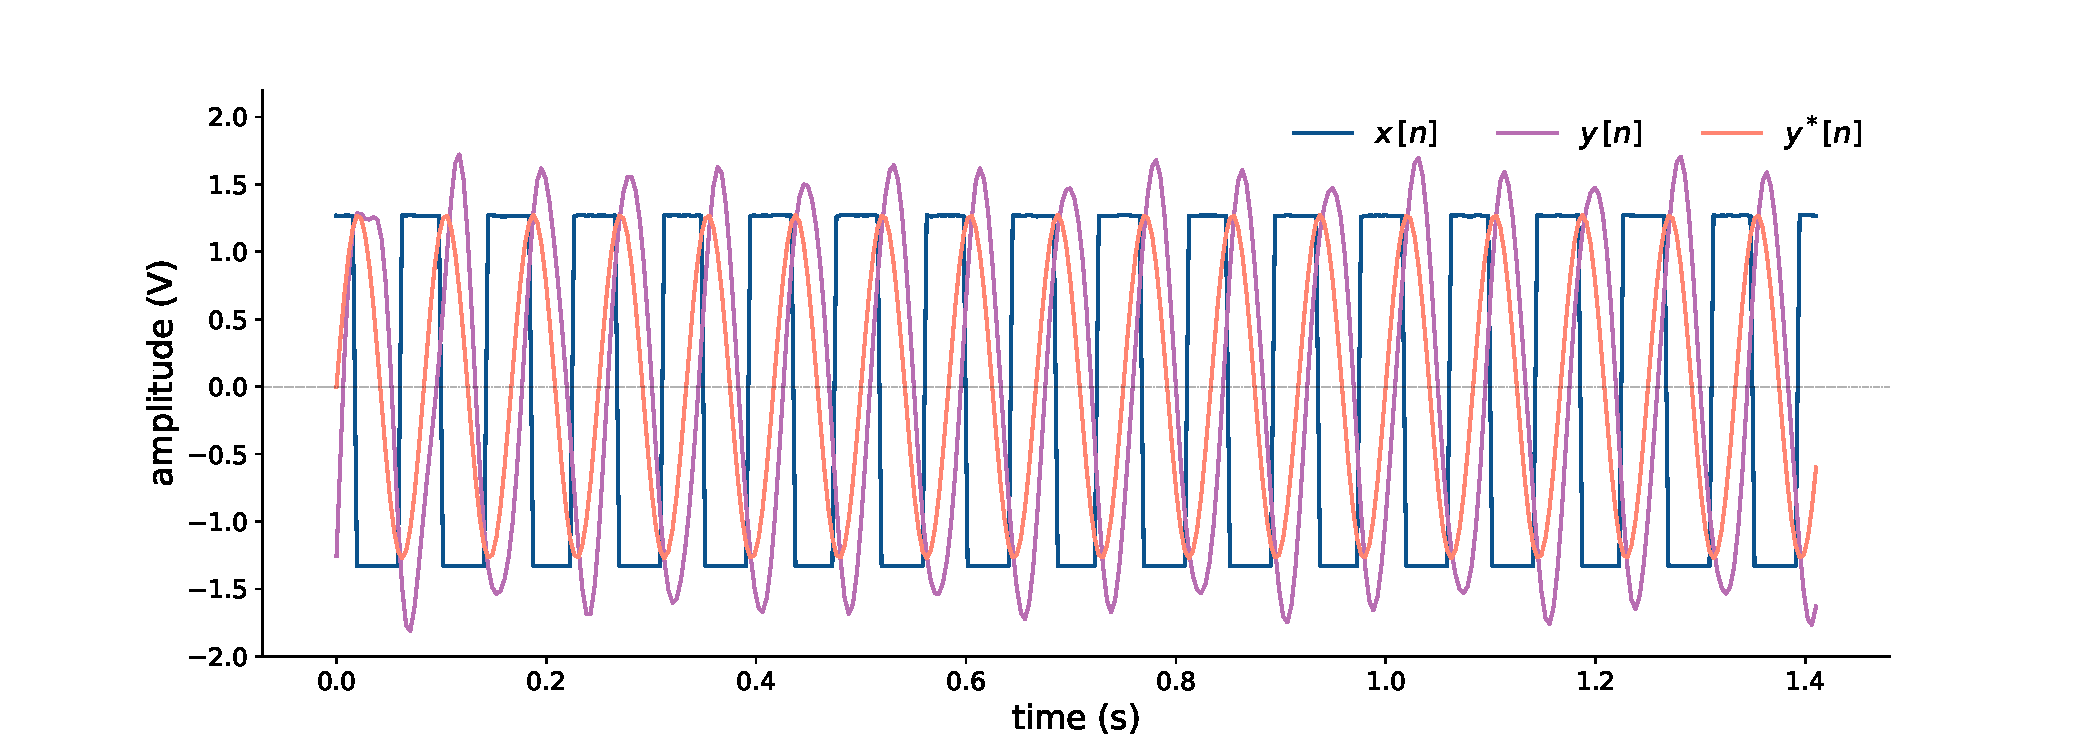
\includegraphics[width=\textwidth]{sq_wave_filtering_time}
    \caption[Time domain plot showing the measured square wave signal together with the digitally-filtered output signal.]{Time domain plot showing the measured square wave signal $x[n]$ together with the digitally-filtered output signal $y[n]$ designed to retain only the fundamental frequency $f_x^{(0)}$ of $x[n]$. The ideal output signal $y^*[n]$ represents a sinsuoid at frequency $f_x^{(0)}$: $y^*[n] = \frac{4}{\pi}\sin(2\pi f_x^{(0)}n)$.}
    \label{fig:sq-wave-time-c6}
\end{figure}

Figure \ref{fig:sq-wave-spectra-c6} shows PSD estimates $\hat{P}_x(\omega)$ and $\hat{P}_y(\omega)$ of $x[n]$ and $y[n]$ respectively in the form of periodograms. Confirming the time domain representation in Figure \ref{fig:sq-wave-time-c6}, $\hat{P}_x(\omega)$ shows power peaks at the odd numbered harmonics of $x[n]$. This can be explained by the Fourier series expansion of an ideal square wave at fundamental frequency $f^{(0)}$ with 50\% duty cycle:
\begin{equation}
    x[n]=\frac{4}{\pi} \sum_{k=1}^{\infty} \frac{\sin (2 \pi(2 k-1) f^{(0)} n)}{2 k-1},
    \label{eq:fourier-series-sinsusoid}
\end{equation}
which is nothing but an infinite sum of sinusoids whose amplitudes decay with frequency. Notice that only odd-numbered harmonics in (\ref{eq:fourier-series-sinsusoid}) are non-zero. Therefore, the ideal spectrum $P_x(\omega)$ of $x[n]$ should be an impulse train at frequencies $(2k-1)f_x^{(0)}, \, k\geq2, \, k\in\mathbb{Z}$. 

While not quite impulses, power peaks of $\hat{P}_x(\omega)$ in Figure \ref{fig:sq-wave-spectra-c6} are clearly visible at the odd-numbered harmonics at 26Hz, 60Hz and so on. The spectrum of the filtered signal, $\hat{P}_y(\omega)$, shows very little distortion in the pass-band between 0 and $f_c=26$Hz, as well as impressively steep roll-off for $f>f_c$. As a result, only the fundamental frequency of $x[n]$ is captured in $y[n]$, as desired. Attenuation of higher frequency harmonics in $x[n]$ by the digital filter is evidently very effective and meets the design criteria stated in Section \ref{subsection:digital-filtering}: stop-band attenuation is approximately 80dB, as can be seen in the power difference between $\hat{P}_x(\omega)$ and $\hat{P}_y(\omega)$ at 60Hz, for example.

\begin{figure}[!htb]
    \centering
    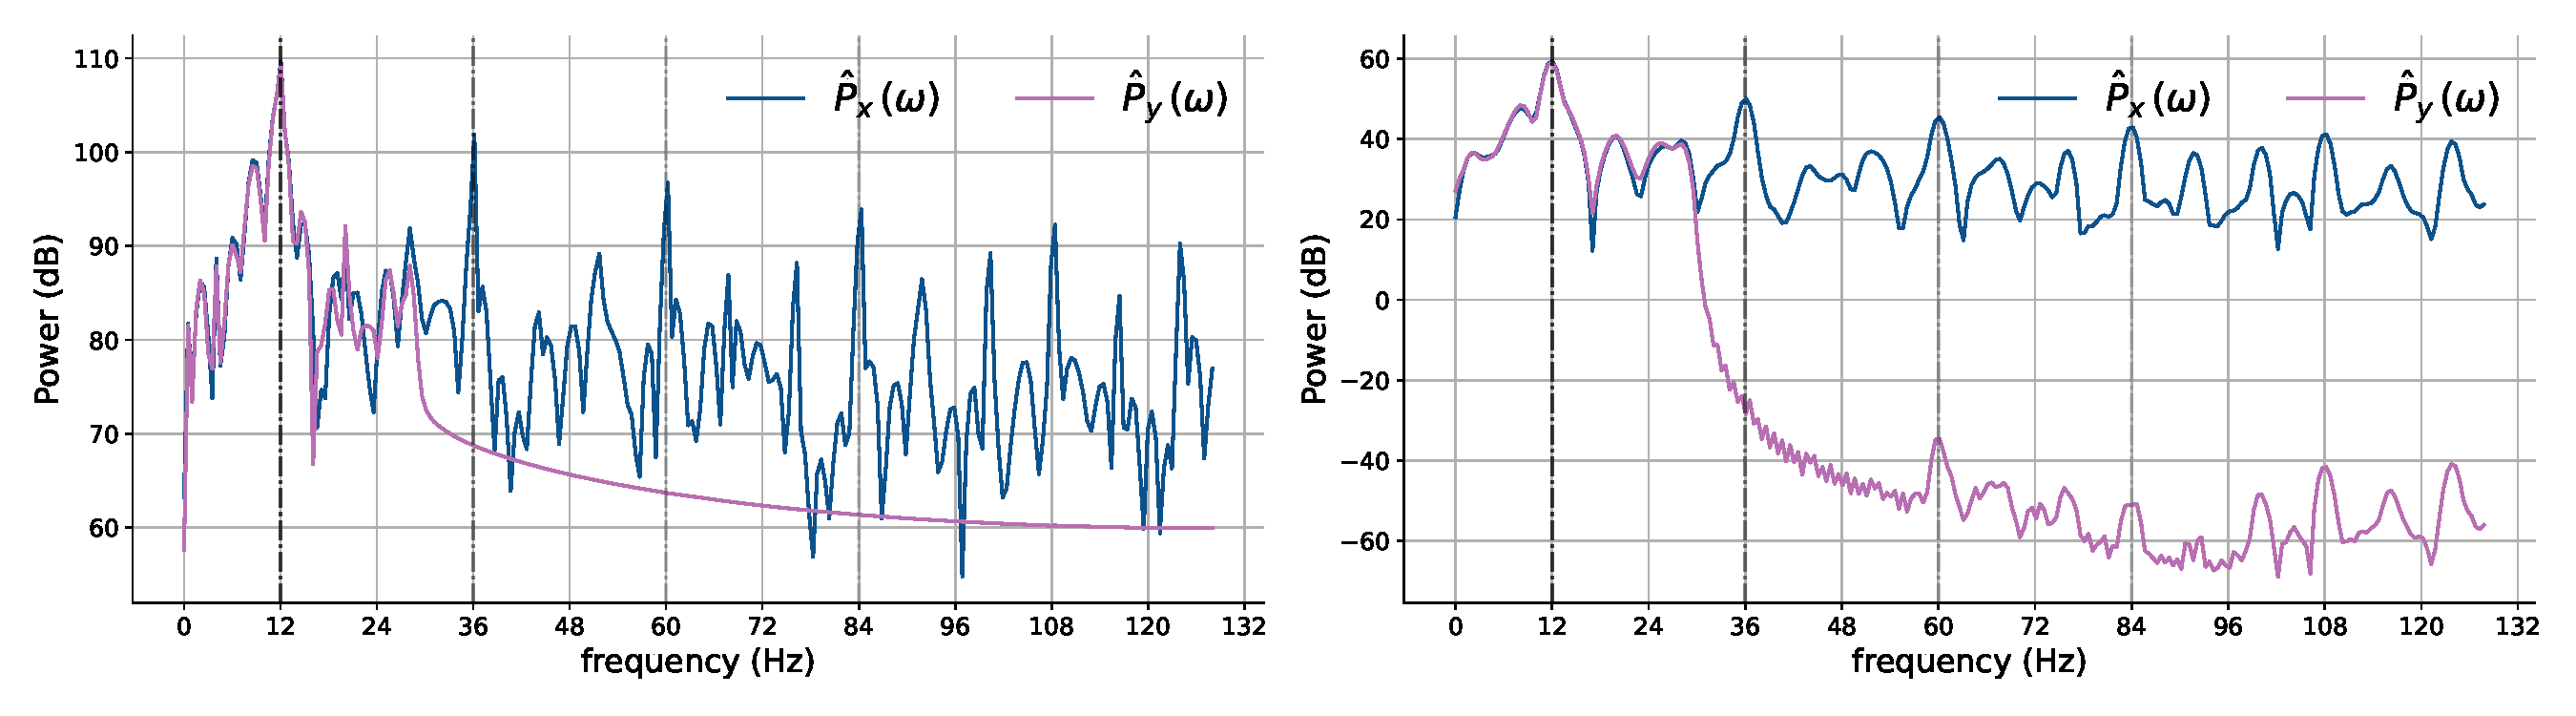
\includegraphics[width=\textwidth]{sq_wave_filtering_spectra}
    \caption[PSD estimates of a measured input signal and its filtered output]{Standard periodogram (left) and Welch-averaged periodogram (right) representing PSD estimates of measured input signal $x[n]$ and filtered output $y[n]$. Dashed vertical lines mark $f_x^{(0)}$ and odd-numbered harmonics of $x[n]$.}
    \label{fig:sq-wave-spectra-c6}
\end{figure}

Along with $\hat{P}_x(\omega)$ as before, Figure \ref{fig:sq-wave-ds-spectra-c6} shows the estimated spectra $\hat{P}_z(\omega)$ and $\hat{P}_\text{alias}(\omega)$ of $z[n]$. $\hat{P}_z(\omega)$ corresponds to the downsampled version of the filtered output $y[n]$ and $\hat{P}_\text{alias}(\omega)$ is the estimated spectrum of $x[n]$ after being downsampled with \textit{no} prior filtering. Both resampled signals were downsampled by a factor of 4 to $f_s'=64$Hz. As is particularly evident from the artefacts at 4Hz, 20Hz and 27Hz in the Welch-averaged periodogram in Figure \ref{fig:sq-wave-ds-spectra-c6}, aliasing has occurred in $\hat{P}_\text{alias}(\omega)$. The full spectrum of $\hat{P}_x(\omega)$ in Figure \ref{fig:sq-wave-spectra-c6} explains this behaviour: $x[n]$ contains substantial energy at higher frequencies past $f>f_n'=32$Hz where $f_n'$ is the Nyquist frequency for the downsampled rate of $f_n'=64$Hz. This demonstrates the necessity for low-pass filtering to isolate the frequency band of interest before downsampling. 
\begin{figure}[h]
    \centering
    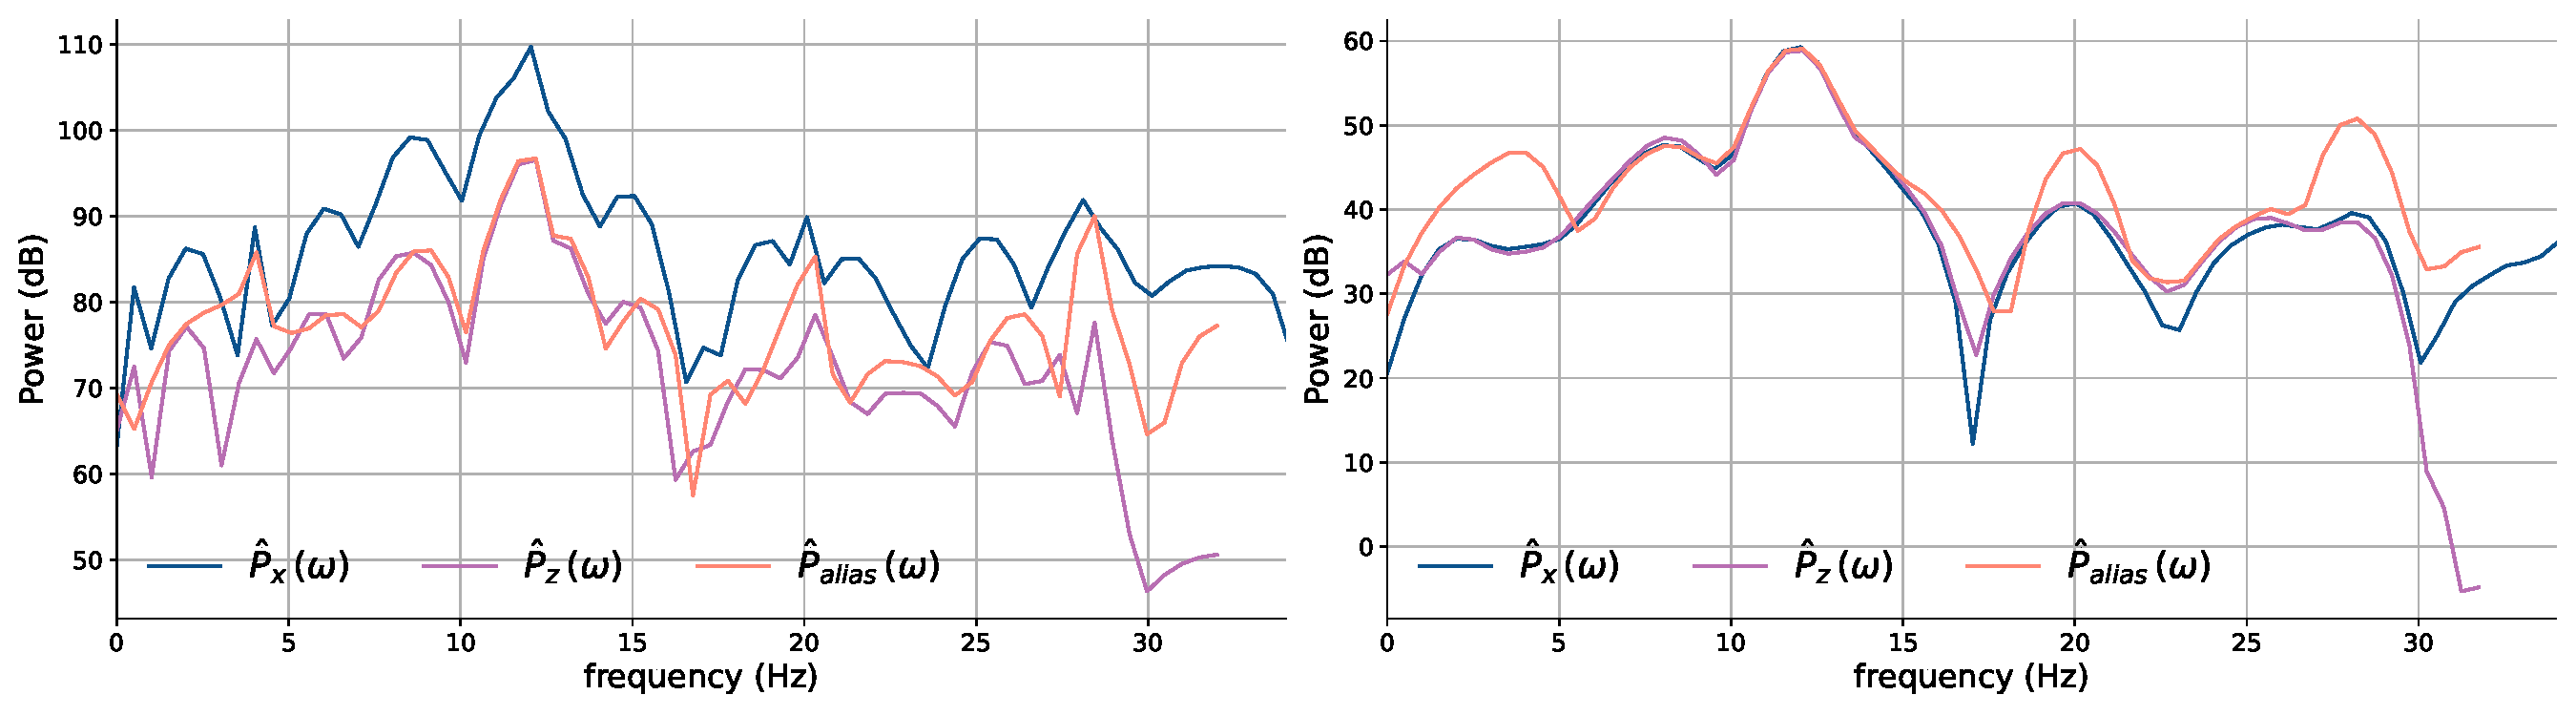
\includegraphics[width=\textwidth]{sq_wave_filtering_ds_spectra}
    \caption[PSD estimates of an input signal, filtered and downsampled version and a downsampled version without filtering.]{Standard periodogram (left) and Welch-averaged periodogram (right) representing PSD estimates $\hat{P}_x(\omega)$ and $\hat{P}_z(\omega)$ of input $x[n]$ and filtered, downsampled output $z[n]$ respectively. $\hat{P}_{\text{alias}}(\omega)$ shows the estimated spectrum of a downsampled version of $x[n]$ \textit{without} prior low-pass filtering}.
    \label{fig:sq-wave-ds-spectra-c6}
\end{figure}
On the other hand, Figure \ref{fig:sq-wave-ds-spectra-c6} also demonstrates the effectiveness of the DSP system as a whole: with suitable low-pass filtering, the spectrum of the downsampled signal $z[n]$ in the pass-band between 0 and 24Hz agrees very closely with that of the original signal $x[n]$. 

\subsection{Hardware and data acquisition}

\begin{figure}[htp]
\subfloat[eyes open]{%
  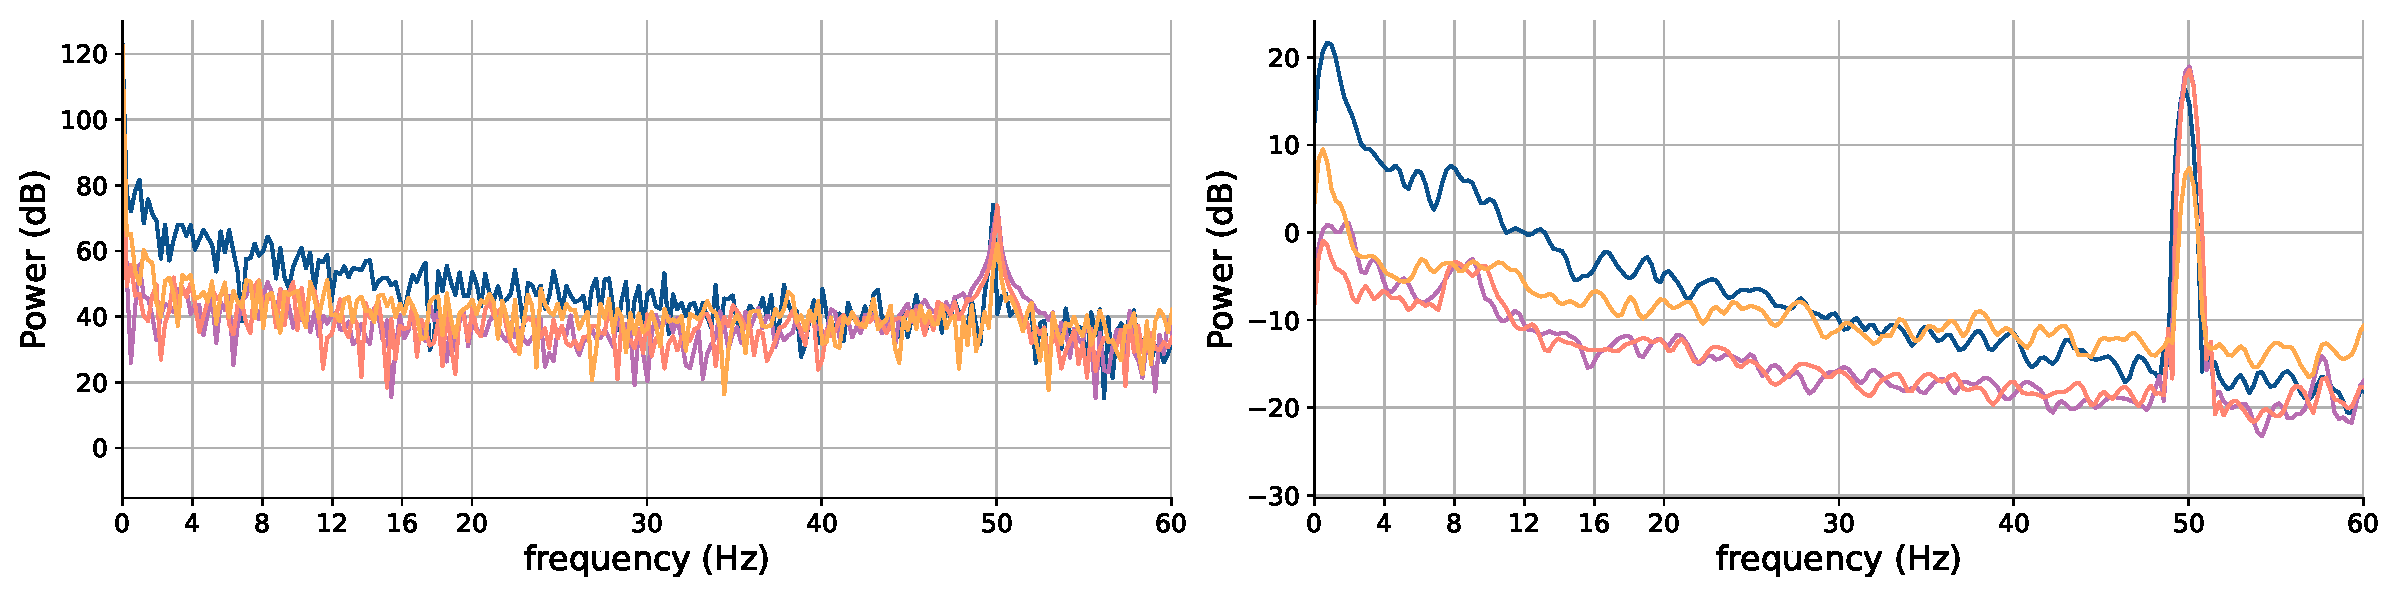
\includegraphics[clip,width=\columnwidth]{eyes_open_alpha_spectra_N1024.pdf}%
}

\subfloat[eyes closed]{%
  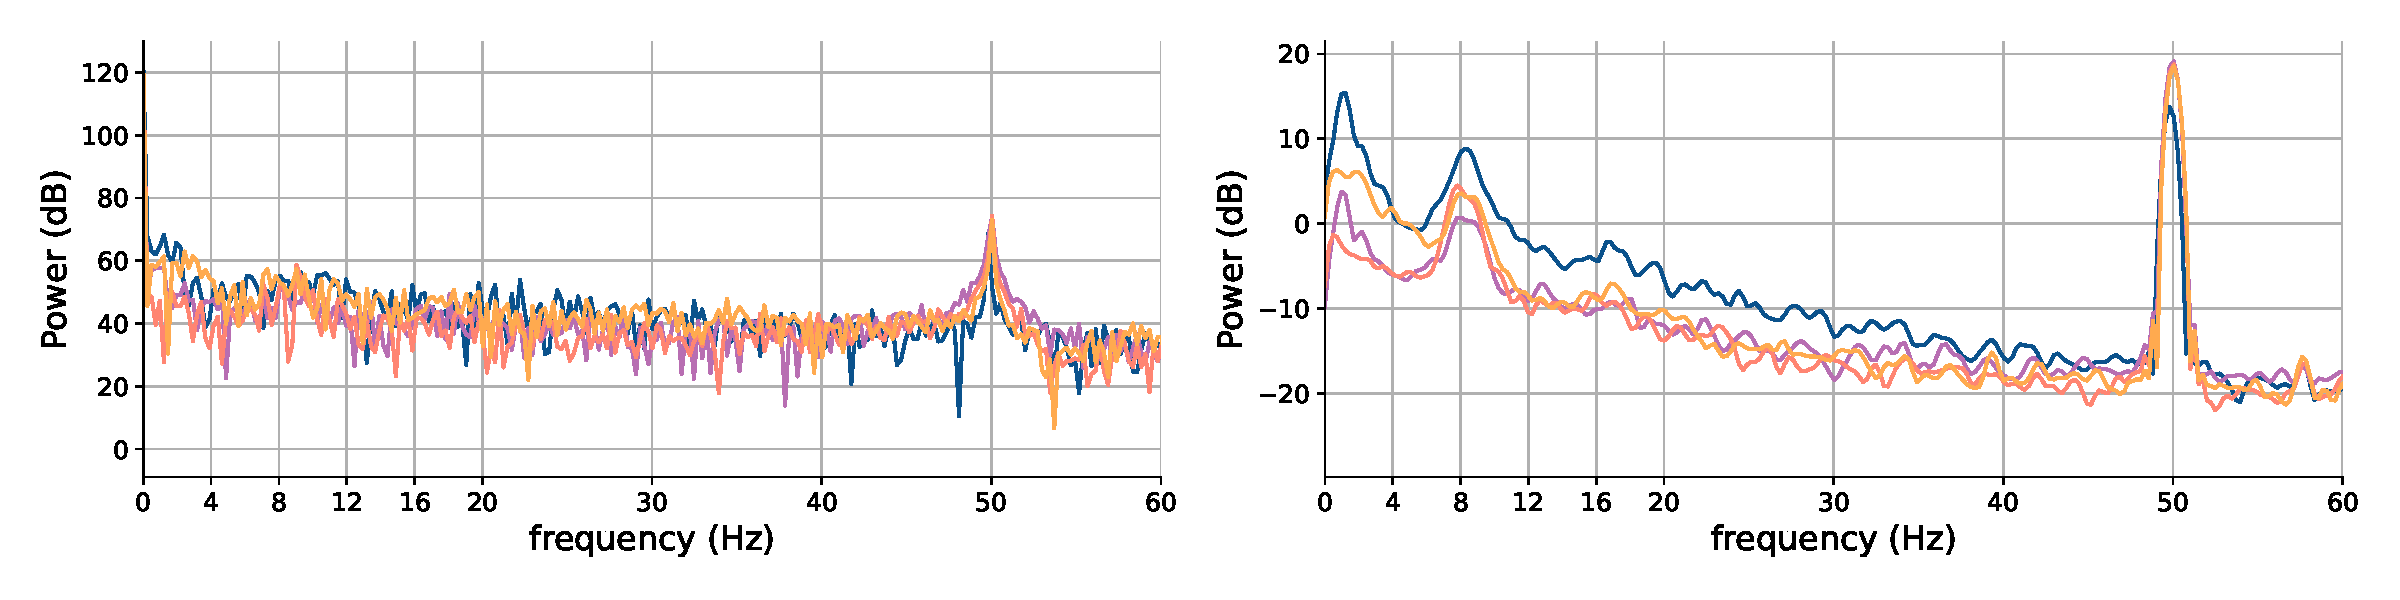
\includegraphics[clip,width=\columnwidth]{eyes_closed_alpha_spectra_N1024.pdf}%
  \label{subfig:alpha-eyes-closed}
}
\caption[Alpha band test: periodograms showing $N=1024$ point PSD estimates for EEG signals measured from a subject in two distinct states: with eyes open and eyes closed.]{\textbf{Alpha band test}: periodograms showing $N=1024$ point PSD estimates for EEG signals measured from a subject in two distinct states: with eyes open and eyes closed. Data was acquired using the early hardware prototype in Figure \ref{fig:frakenstein-hardware}. Attention should be given to signal power around $8-10$Hz (alpha band). In both (a) and (b), the left subplot shows a standard, non-windowed periodogram accompanied by a Welch-averaged periodogram to the right. Different coloured traces represent independent trials.}
\label{fig:alpha-periodograms}
\end{figure}

As mentioned in Chapter \ref{chapter:experimental-procedure}, the rudimentary headband discussed in Section \ref{subsection:mech-hardware-frankenstein} was created as a means of acquiring and testing real-life data from the electronic hardware prototype introduced in Section \ref{subsection:electronic-hardware-proto}. After verifying the fidelity of the DSP system, a basic BCI test known as the 'alpha test' was performed. This involves measuring the EEG signals generated by the brain's visual cortex during two distinct states: with eyes open and eyes closed. In particularly, signal energy in the alpha band between 8-12Hz is observed. As mentioned briefly in Section \ref{subsection:nature-of-eeg-signals}, a working BCI should be able to discern greater energy in the alpha band when a subject's eyes are closed compared to when open.

Figure \ref{fig:alpha-periodograms} shows the estimated power spectra recorded over several trials in each of the two aforementioned states. Particularly around 8Hz, Subfigure \ref{subfig:alpha-eyes-closed} representing the eyes closed state shows noticeably more signal power in the alpha band relative to the rest of the signal (compared to the eyes open state). This is suggestive of the presence of valid EEG signals as opposed to just random noise.

\subsection{Execution time profiling}
A number of trials were performed to determine the consistency of execution time across key system processes in the sample-decode-publish loop. Figure \ref{fig:timing-distributions} shows the distributions of execution times recorded over several trials. In each trial, all possible functionality was enabled so as to test maximum computational loading. "Auxiliarly processing time" is defined as the processing time in each loop required for any operations \textit{besides} decoding computation and publishing to AWS over MQTT. 

\begin{figure}[htp]
\centering
\subfloat[decoding computation]{%
  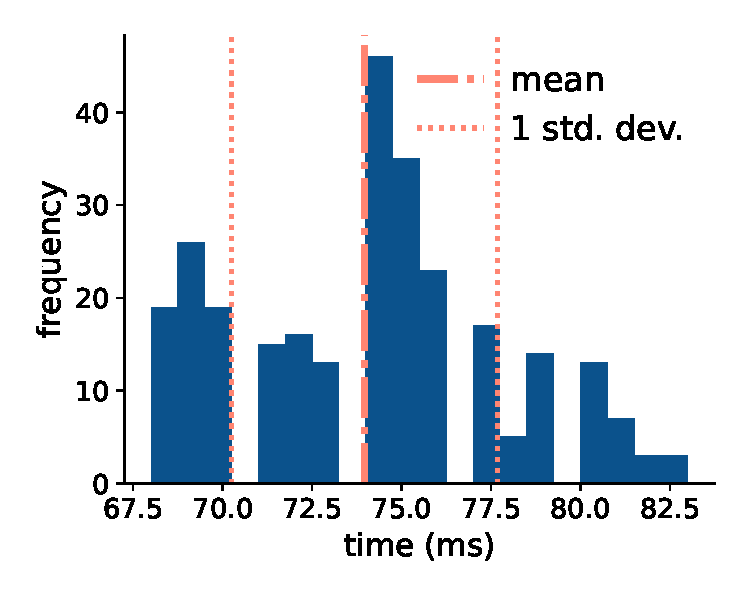
\includegraphics[clip,width=0.3\columnwidth]{report/C6 Results/assets/comp_tim_distr.pdf}%
  \label{subfig:timing-comp}
}
\hfill
\subfloat[MQTT publish]{%
  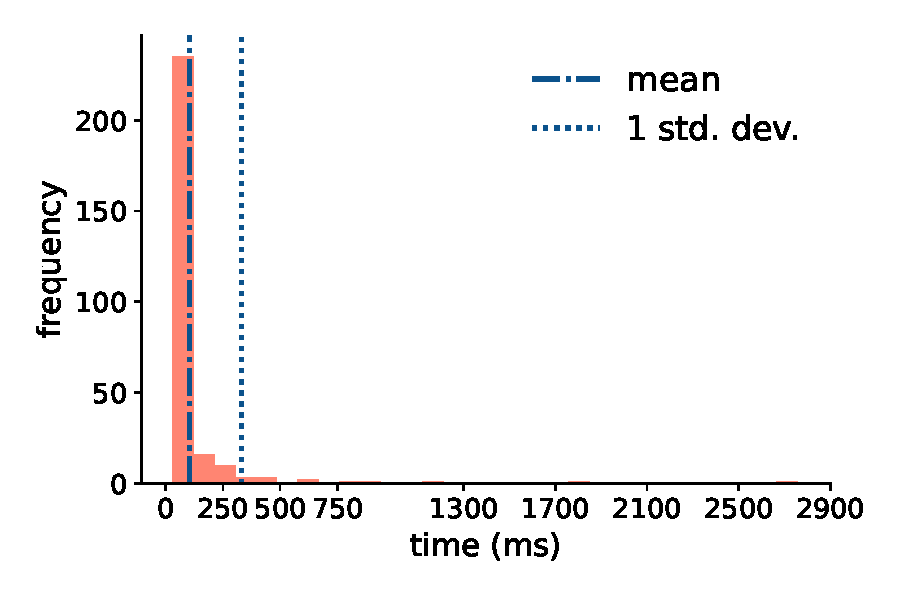
\includegraphics[clip,width=0.36\columnwidth]{report/C6 Results/assets/pub_tim_distr.pdf}%
  \label{subfig:timing-pub}
}
\hfill 
\subfloat[auxiliary processing]{%
  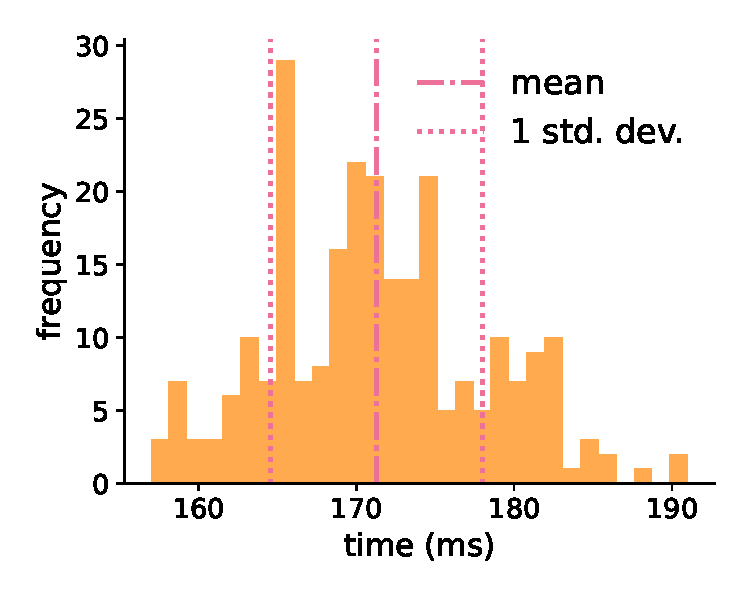
\includegraphics[clip,width=0.3\columnwidth]{report/C6 Results/assets/aux_proc_tim_distr.pdf}%
  \label{subfig:timing-aux}
}
\caption[Execution time distributions for key processes in the sample-decode-publish loop.]{Execution time distributions for key processes in the sample-decode-publish loop. Auxiliary processing refers to any processing besides that which is required for decoding and publishing data over MQTT.}
\label{fig:timing-distributions}
\end{figure}


\section{Experimental Decoding Results}
In this section, the experimental results of various decoding algorithms introduced in Chapter \ref{chapter:lit-review} are reported. Unfortunately, because only single channel EEG signals were available using the hardware provided in this project, the TRCA algorithm was no longer appropriate. This is due to the fact that it tries to find optimal \textit{spatial} filters for task-related discrimination; effectively optimally-weighted combinations of multiple channels. Clearly, having only a single channel renders this approach ineffective. 

The decoding results of the CCA algorithm are presented briefly, however, greater attention is paid to those of the GCCA and MsetCCA algorithms. The latter two algorithms use data from across trials to form a `reference template' in addition to the ordinary CCA method that only compares measured signals with the artificially-constructed sinusoidal reference set. 

\subsubsection{Evaluation of results}
\label{subsection:evaluating-results}
Worth noting is the method used to evaluate results reported below. For template-based decoding algorithms (GCCA, MsetCCA), initial training or calibration is required using historical template data. The term `calibration' is preferred since in practice, calibration must happen automatically on the device and the term `training' is typically associated with offline model fitting.

Leave-$p$-out cross-validation (LpO CV) was employed in order to minimise the risk of selection bias or overfitting to pathological test cases. Usually, LpO CV refers to \textit{training} a model on $n-p$ observations and \textit{validating} on the held-out $p$ validations (with $p<n$). However, in this project, template-based algorithms were instead \textit{calibrated} on the smaller $p$-partition and validated on the remaining $n-p$ samples. This more appropriately reflects the practical dynamic of this system where only few calibration trials will be available before inference needs to begin.

LpO CV was selected, as opposed to leave-one-out CV\footnote{a special case of LpO CV with $p=1$ that is more commonly used}, for example, as it provides the ability to vary $p$ in order to investigate the effect of more or fewer calibration trials on decoding performance. For $n$ trials or observations, LpO CV will generate $\binom{n}{p}$ unique calibration-validation splits\footnote{This would generally become computationally infeasible for even modest $n$. However, the calibration or `training' processes for the algorithms in this project were not computationally intensive and the number of trials in each experiment never exceeded 10.}. Validation metrics, such as accuracy, are then averaged across all splits (unless otherwise stated). This is depicted more graphically in Figure \ref{fig:lpocv-diagram}.
\begin{figure}[h]
    \centering
    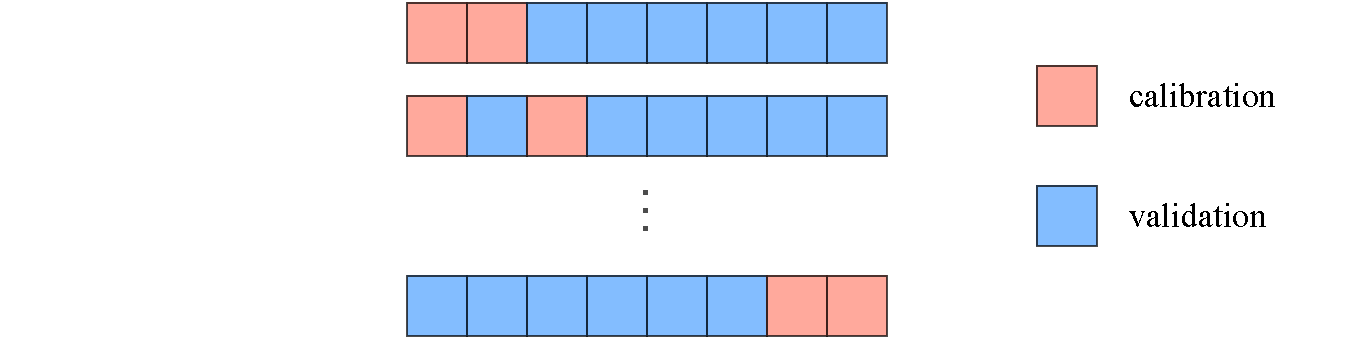
\includegraphics[width=0.65\textwidth]{LpoCV}
    \caption[Leave-$p$-out cross validation (Lpo CV)]{Diagram illustrating leave-$p$-out cross validation (Lpo CV). Individual blocks in each row are different trials, each represented by a data matrix $X_n\in\R^{N_s\times N_c}$ where $N_s$ is the number of samples per trial and $N_c$ is the number of channels ($N_c=1$ in this project). For $n$ trials, there will be $\binom{n}{p}$ different calibration-validation splits (rows of blocks).}
    \label{fig:lpocv-diagram}
\end{figure}
Note that, contrary to Lpo CV, the more well-known k-fold cross-validation technique is a \textit{non-exhaustive} CV method as it does not test every combination of splits in the original data sample: it only selects train-validation splits whose elements are contiguous. In comparison, Lpo CV may select non-contiguous elements in either or both of the train and validation sets. Therefore, k-fold CV is a less computationally-intensive approximation of the more rigorous Lpo CV method. 

\subsection{The effect of recording window length}
\label{subsection:decoding-acc-ns-effect}
As alluded to in Section \ref{subsection:time-frequency-considerations-c2}, arguably the most important factor in the decoding system - besides the actual algorithm used - is the length of the recording window $T$. As cited in the literature review, decoding accuracy almost always improved with increasing $T$. This is expected; longer time windows offer more samples to the decoding algorithm being used. However, the trade off is decreased information transfer rate (ITR) which results in a more sluggish BCI system. 

Figures \ref{fig:gcca-acc-ns} and \ref{fig:mset-acc-ns} show the effect of varying $T$ on decoding accuracy for the GCCA and MsetCCA algorithms respectively. For each algorithm, the effect of varying $T$ is tested with four different calibration scenarios with $p=1,\dots,4$ where $p$ is the number of training or calibration trials. As expected, there is a monotonic increase in \textit{average} decoding accuracy (across stimulus frequencies for each trial) with increasing $T$. Clearly, there is also an interaction with the number of calibration trials $p$.

%% [SAMPLING LENGTH] Experiments with varying Ns: GCCA
\begin{figure}[htp]
\subfloat[$p=1$]{%
    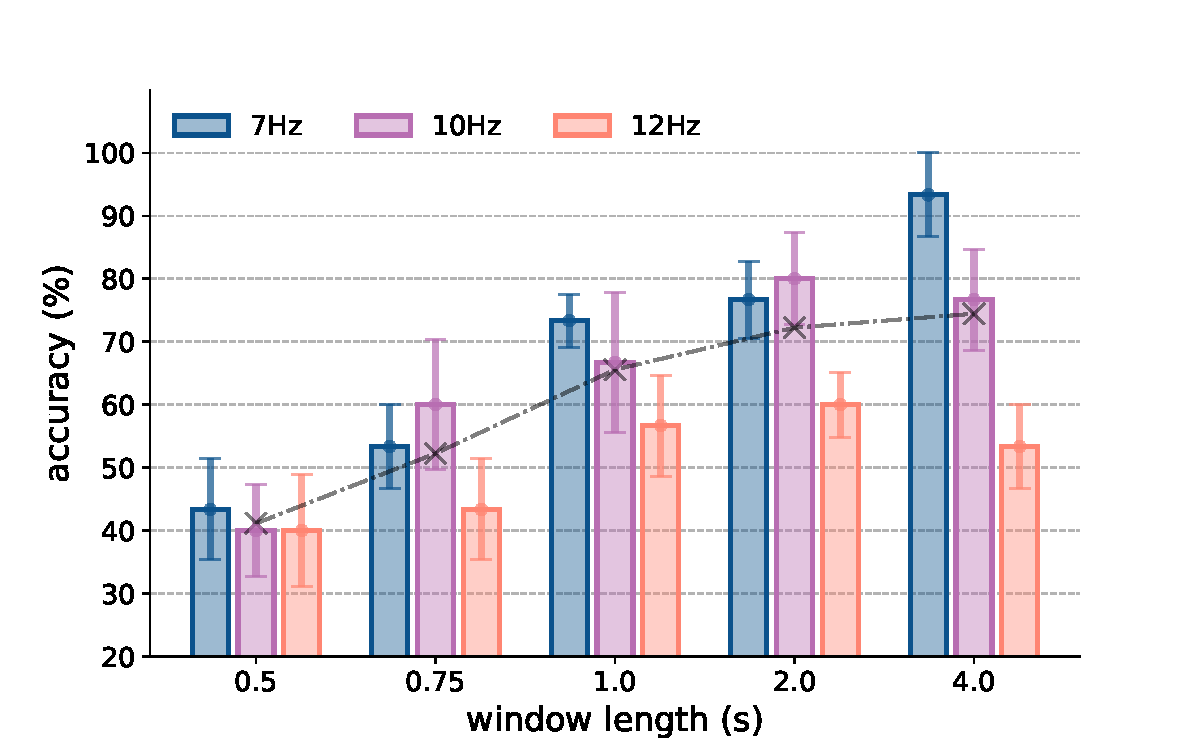
\includegraphics[clip,width=0.49\columnwidth]{report/C6 Results/assets/acc_Ns_gcca_Nt1.pdf}%
    \label{subfig:gcca-ns-nt1}
}
\hfill
\subfloat[$p=2$]{%
    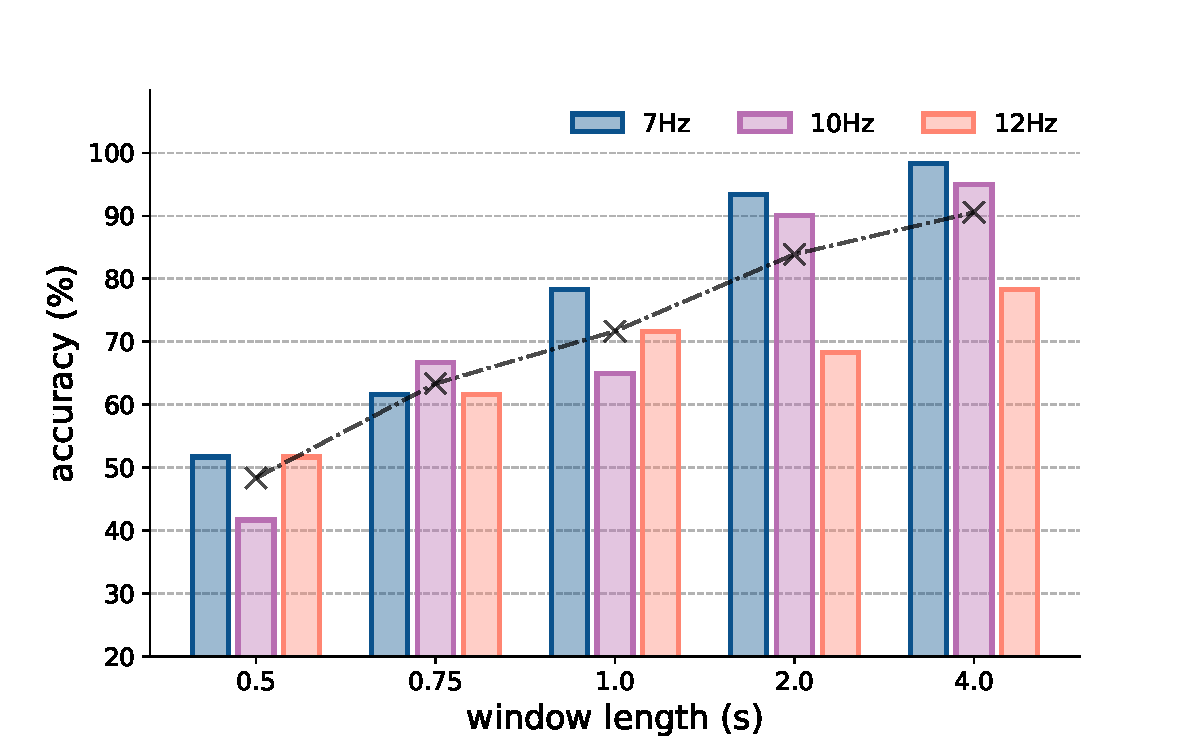
\includegraphics[clip,width=0.49\columnwidth]{report/C6 Results/assets/acc_Ns_gcca_Nt2.pdf}%
    \label{subfig:gcca-ns-nt2}
}
% ensure there is a space below here!

% \vspace{-0.5cm}
\subfloat[$p=3$]{%
    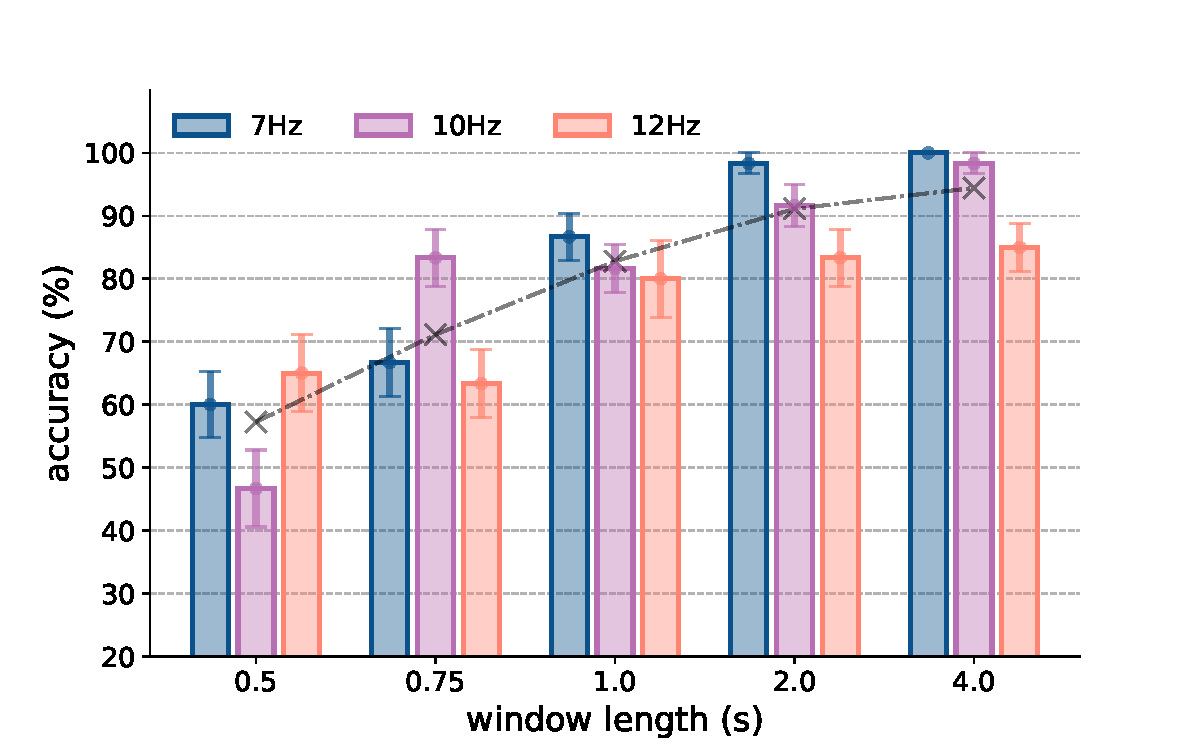
\includegraphics[clip,width=0.49\columnwidth]{report/C6 Results/assets/acc_Ns_gcca_Nt3.pdf}%
    \label{subfig:gcca-ns-nt3}
}
\hfill
\subfloat[$p=4$]{%
    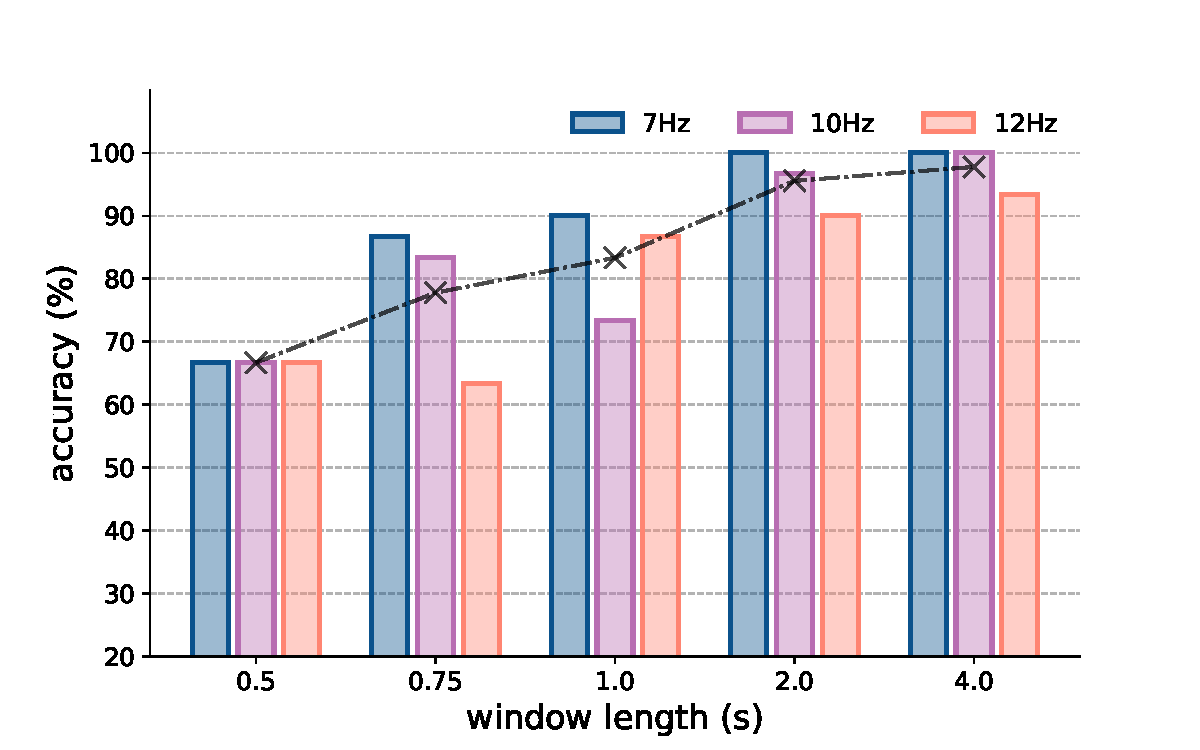
\includegraphics[clip,width=0.49\columnwidth]{report/C6 Results/assets/acc_Ns_gcca_Nt4.pdf}%
    \label{subfig:gcca-ns-nt4}
}

\caption[GCCA decoding accuracy, varying $T$: effect of varying recording window length $T$ on validation accuracy for different numbers of calibration trials $p$]{\textbf{GCCA decoding accuracy, varying }$T$: effect of varying recording window length $T$ on validation accuracy for different numbers of calibration trails $N_t$. In each subfigure, all results were computed using $p=n, \, n\in\{1, \dots, 4\}$ calibration trials. Crosses connected with dashed traces denote average decoding accuracy across stimulus frequencies for a given a given window length $T$. Error bars denote one standard error of the mean.}
\label{fig:gcca-acc-ns}
\end{figure}

%% [SAMPLING LENGTH] Experiments with varying Ns: MsetCCA
\begin{figure}[htp]
\subfloat[$p=1$]{%
    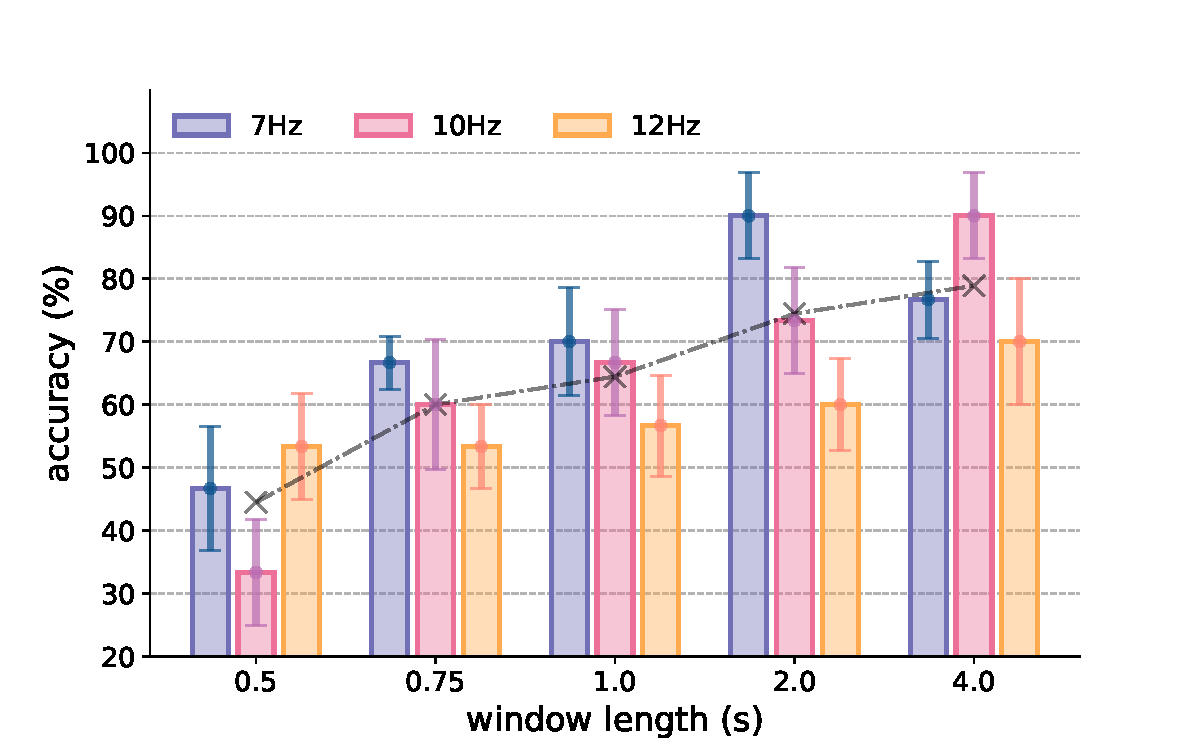
\includegraphics[clip,width=0.49\columnwidth]{report/C6 Results/assets/acc_Ns_mcca_Nt1.pdf}%
    \label{subfig:mcca-ns-nt1}
}
\hfill
\subfloat[$p=2$]{%
    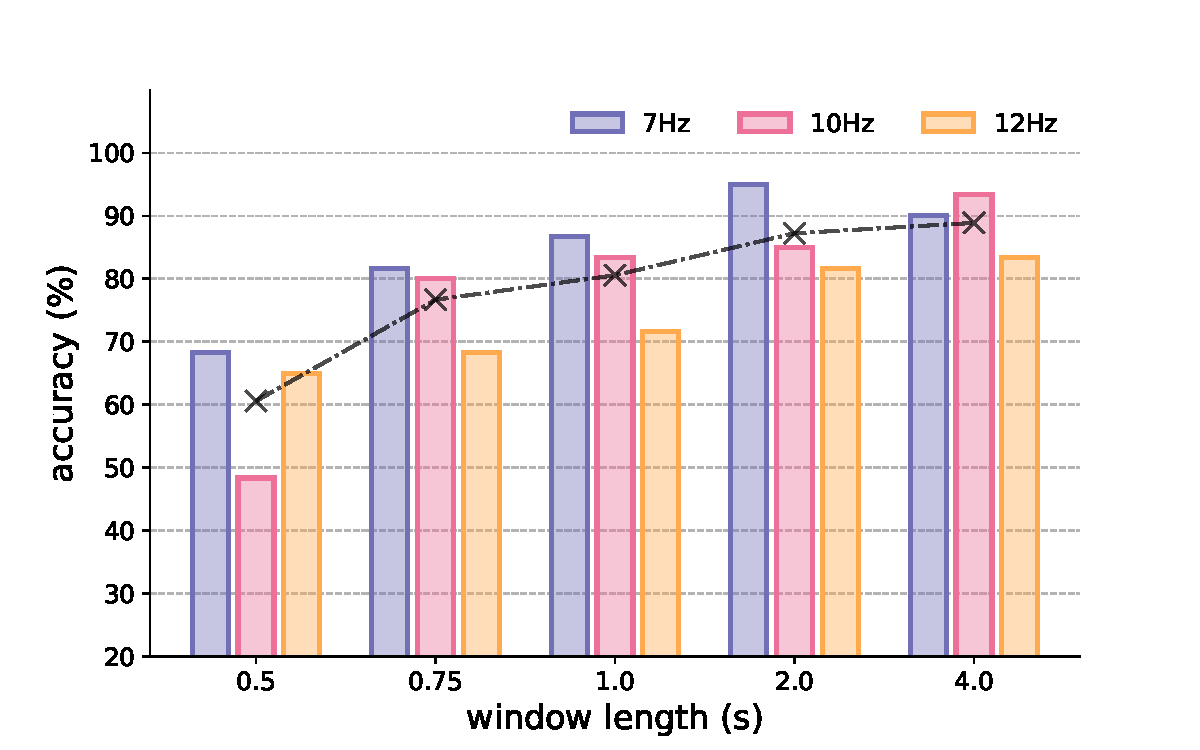
\includegraphics[clip,width=0.49\columnwidth]{report/C6 Results/assets/acc_Ns_mcca_Nt2.pdf}%
    \label{subfig:mcca-ns-nt2}
}
% ensure there is a space below here!

\subfloat[$p=3$)]{%
    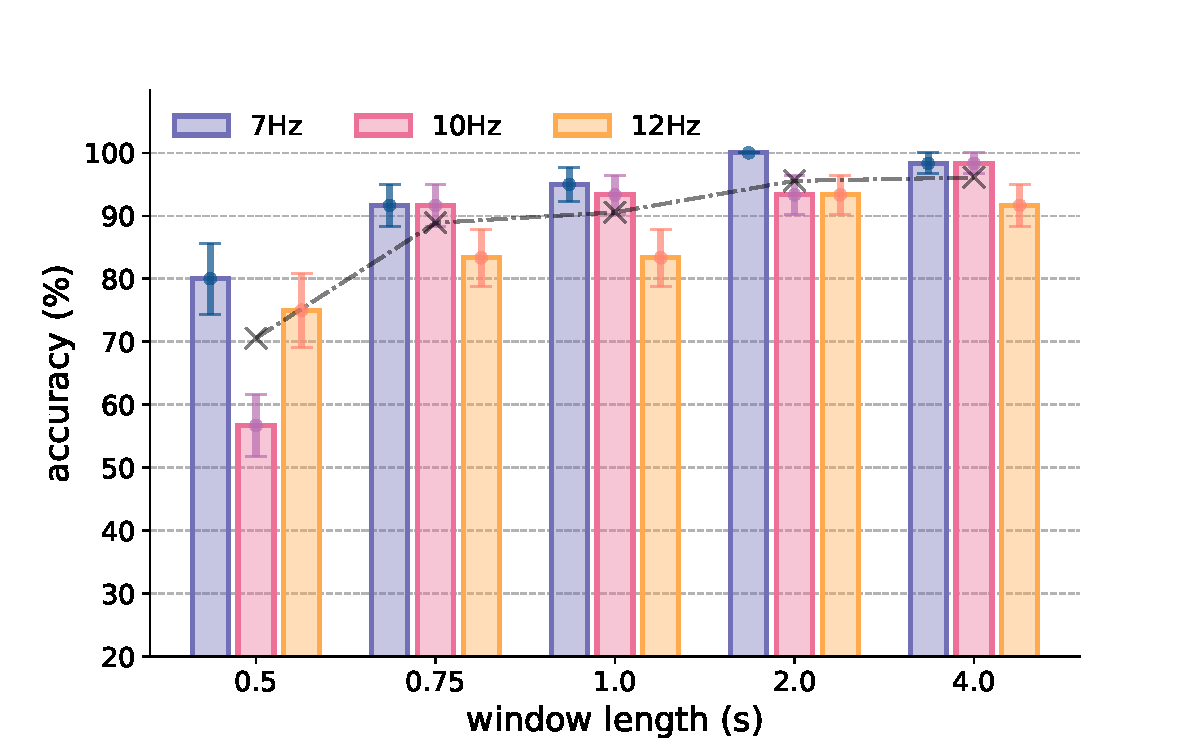
\includegraphics[clip,width=0.49\columnwidth]{report/C6 Results/assets/acc_Ns_mcca_Nt3.pdf}%
    \label{subfig:mcca-ns-nt3}
}
\hfill
\subfloat[$p=4$]{%
    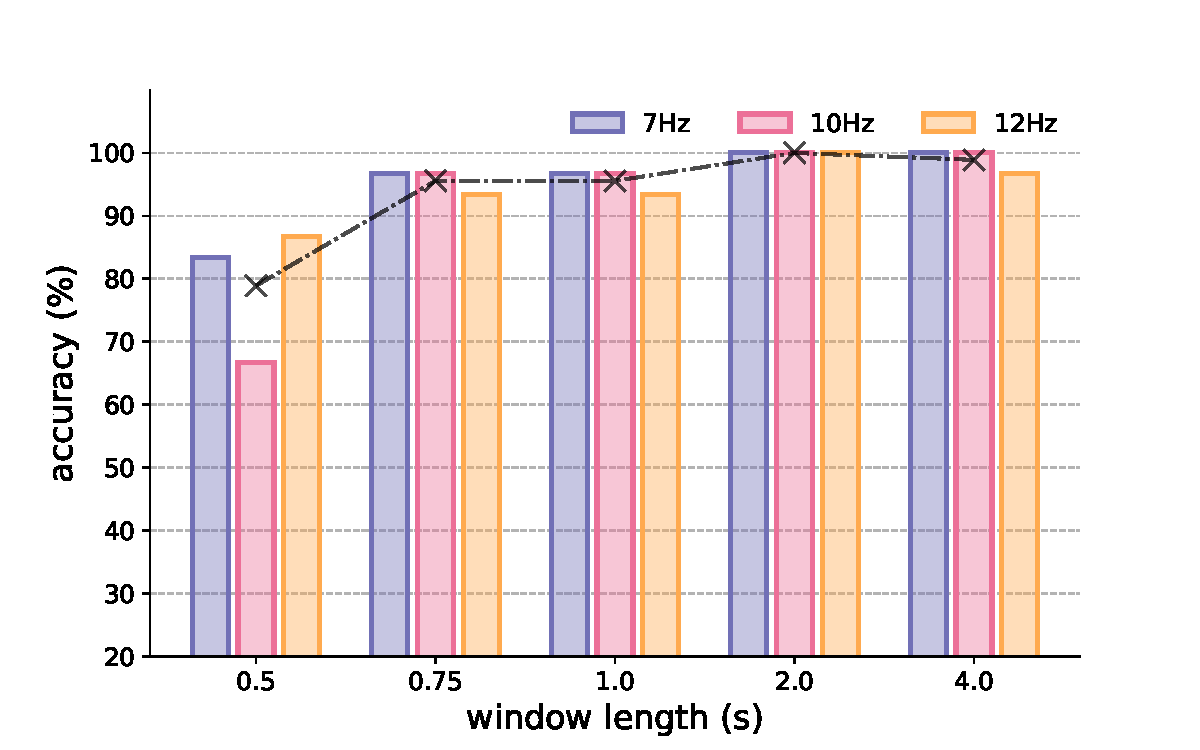
\includegraphics[clip,width=0.49\columnwidth]{report/C6 Results/assets/acc_Ns_mcca_Nt4.pdf}%
    \label{subfig:mcca-ns-nt4}
}

\caption[MsetCCA decoding accuracy, varying $T$: effect of varying recording window length $T$ on validation accuracy for different numbers of calibration trails $p$]{\textbf{MsetCCA decoding accuracy, varying }$T$: effect of varying recording window length $T$ on validation accuracy for different numbers of calibration trails $p$. In each subfigure, all results were computed using $p=n, \, n\in\{1, \dots, 4\}$ calibration trials. Crosses connected with dashed traces denote average decoding accuracy across stimulus frequencies for a given a given window length $T$. Error bars denote one standard error of the mean.}
\label{fig:mcca-acc-ns}
\end{figure}

\subsection{The effect of varying calibration trials}
\label{subsection:decoding-acc-ntr-effect}
Another important consideration for template-based algorithms such as GCCA and MsetCCA cited in the literature is the number of calibration or training trials used to `fit' the algorithms prior to inference. In this context, `fit' refers to computing optimised reference signals or canonical weights based on historical data. 

Figures \ref{fig:gcca-acc-nt} and \ref{fig:mset-acc-nt} show the effect of varying $p$, the number of calibration trials used to fit the GCCA and MsetCCA algorithms respectively. These tests were performed in four different sets, each with a distinct recording window length $T$. Similar to the prior experiment for varying $T$ directly, there is a monotonic increase in \textit{average} decoding accuracy with increasing $p$. Note that the same cross-validation evaluation procedure as explained in Section \ref{subsection:evaluating-results} was used to generate these results.

%% Experiments with varying Nt: GCCA
\begin{figure}[htp]
\subfloat[$T = 0.75$s ($N_s=192, N_s'=48$)]{%
    \label{subfig:gcca-nt-ns48}
    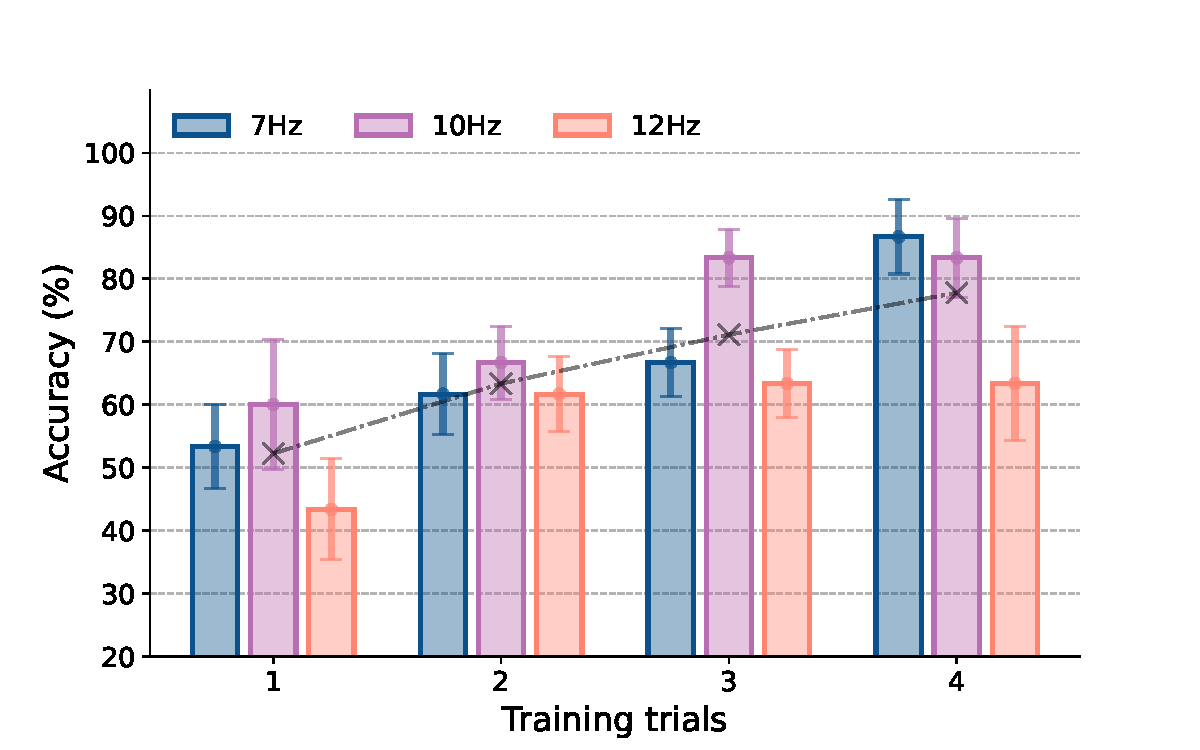
\includegraphics[clip,width=0.49\columnwidth]{report/C6 Results/assets/acc_Nt_gcca_Ns48.pdf}%
}
\hfill
\subfloat[$T = 2$s ($N_s=512, N_s'=128$)]{%
    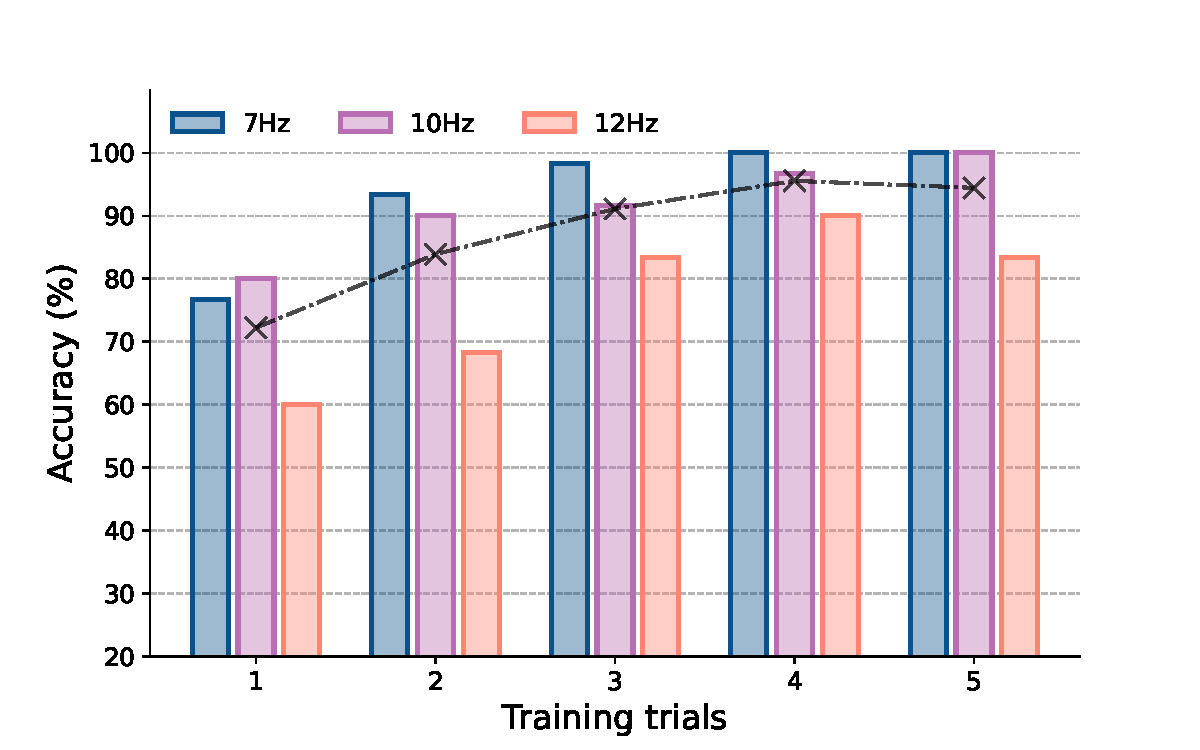
\includegraphics[clip,width=0.49\columnwidth]{report/C6 Results/assets/acc_Nt_gcca_Ns128.pdf}%
    \label{subfig:gcca-nt-ns128}
}
% ensure there is a space below here!

% \subfloat[$T = 2$s ($N_s=512, N_s'=128$)]{%
%     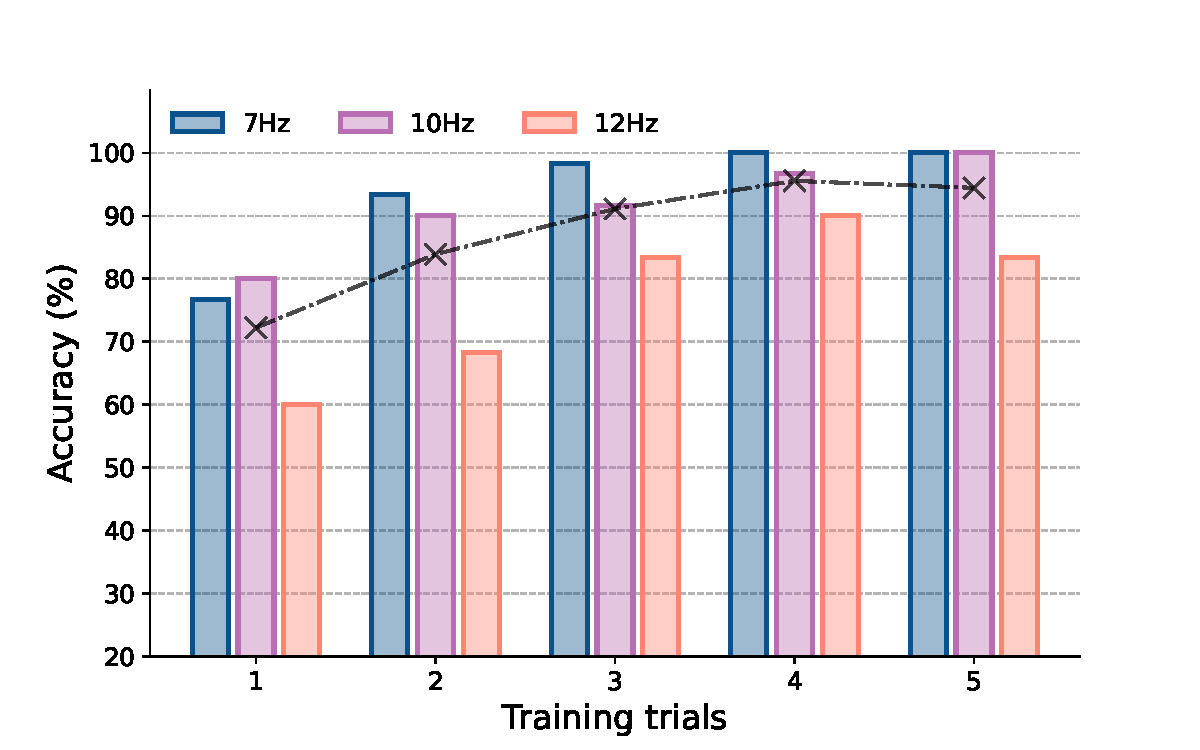
\includegraphics[clip,width=0.49\columnwidth]{report/C6 Results/assets/acc_Nt_gcca_Ns128.pdf}%
%     \label{subfig:gcca-nt-ns128}
% }
% \hfill
% \subfloat[$T = 4$s ($N_s=1024, N_s'=256$)]{%
%     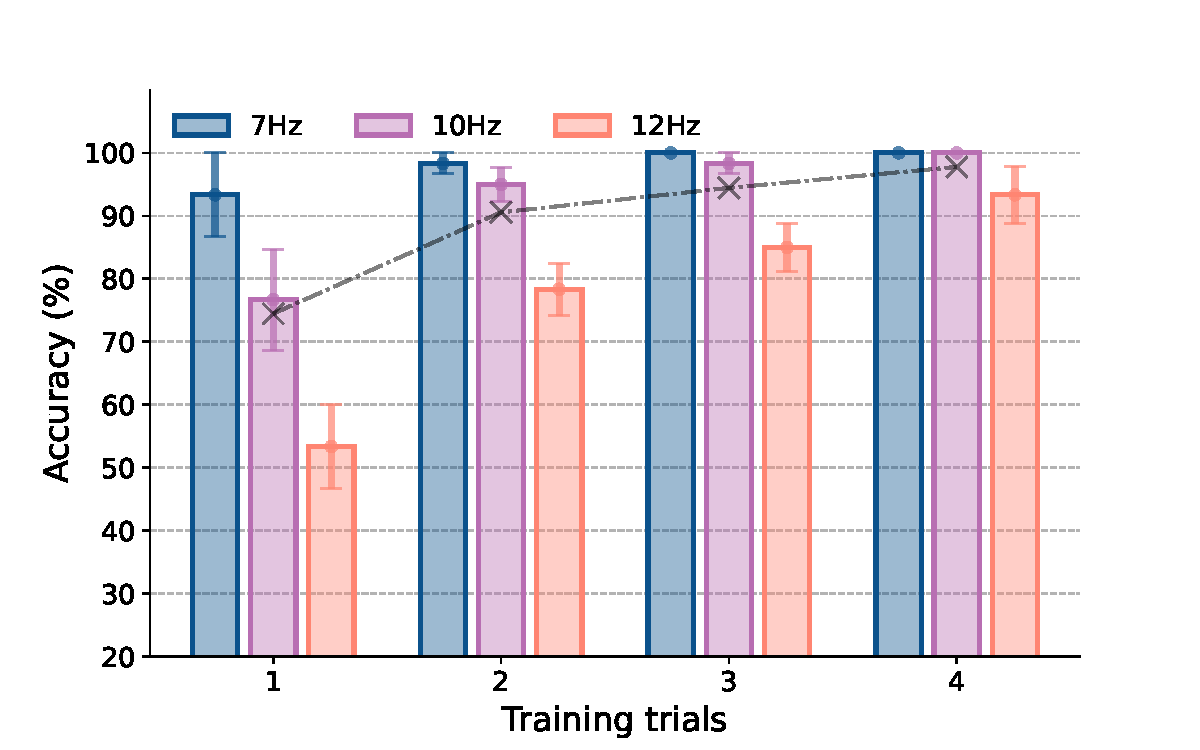
\includegraphics[clip,width=0.49\columnwidth]{report/C6 Results/assets/acc_Nt_gcca_Ns256.pdf}%
%     \label{subfig:gcca-nt-ns256}
% }
\caption[GCCA decoding accuracy, varying $p$: effect of varying the number of training (calibration) trials $p$ on validation accuracy for recording windows of varying length $T$.]{\textbf{GCCA decoding accuracy, varying }$p$: effect of varying the number of training (calibration) trials $p$ on validation accuracy for recording windows of varying length $T$. In each subfigure, all trials are of equal length $T$ seconds which equates to $N_s$ samples at $f_s=256$Hz and $N_s'$ samples at the downsampled rate of $f_s'=64$Hz. Crosses connected with dashed traces denote average decoding accuracy across stimulus frequencies for a given $p=n, \, n\in\{1, \dots, 5\}$. Error bars denote one standard error of the mean.}
\label{fig:gcca-acc-nt}
\end{figure}


%% Experiments with varying Nt: MsetCCA
\begin{figure}[htp]
\subfloat[$T = 0.75$s ($N_s=192, N_s'=48$)]{%
    \label{subfig:gcca-nt-ns48}
    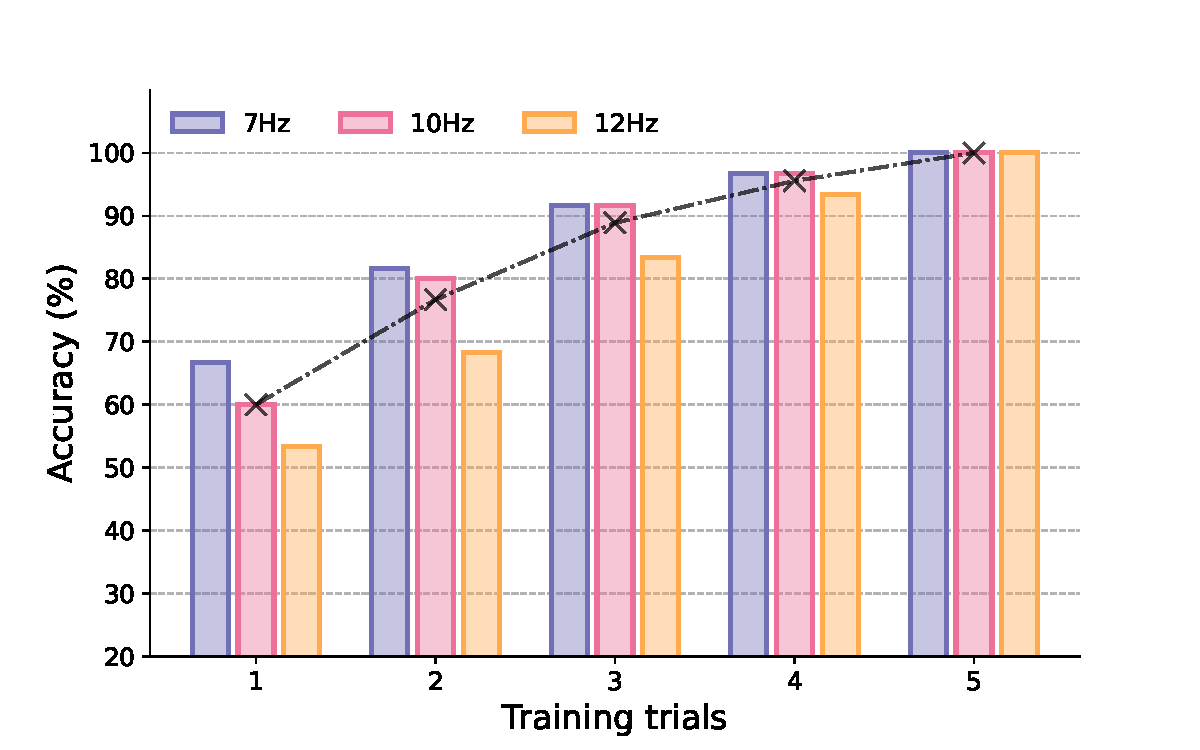
\includegraphics[clip,width=0.49\columnwidth]{report/C6 Results/assets/acc_Nt_mcca_Ns48.pdf}%
}
\hfill
\subfloat[$T = 2$s ($N_s=512, N_s'=128$)]{%
    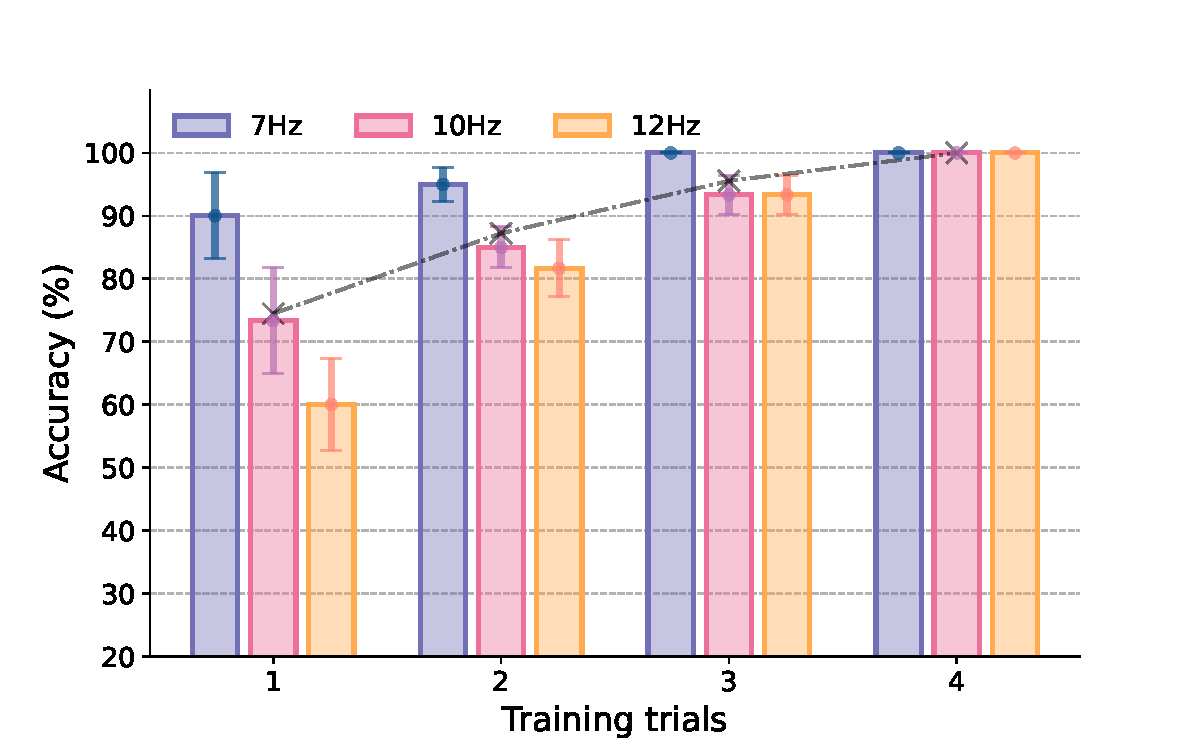
\includegraphics[clip,width=0.49\columnwidth]{report/C6 Results/assets/acc_Nt_mcca_Ns128.pdf}%
    \label{subfig:mset-nt-ns128}
}
% ensure there is a space below here!

% \subfloat[$T = 2$s ($N_s=512, N_s'=128$)]{%
%     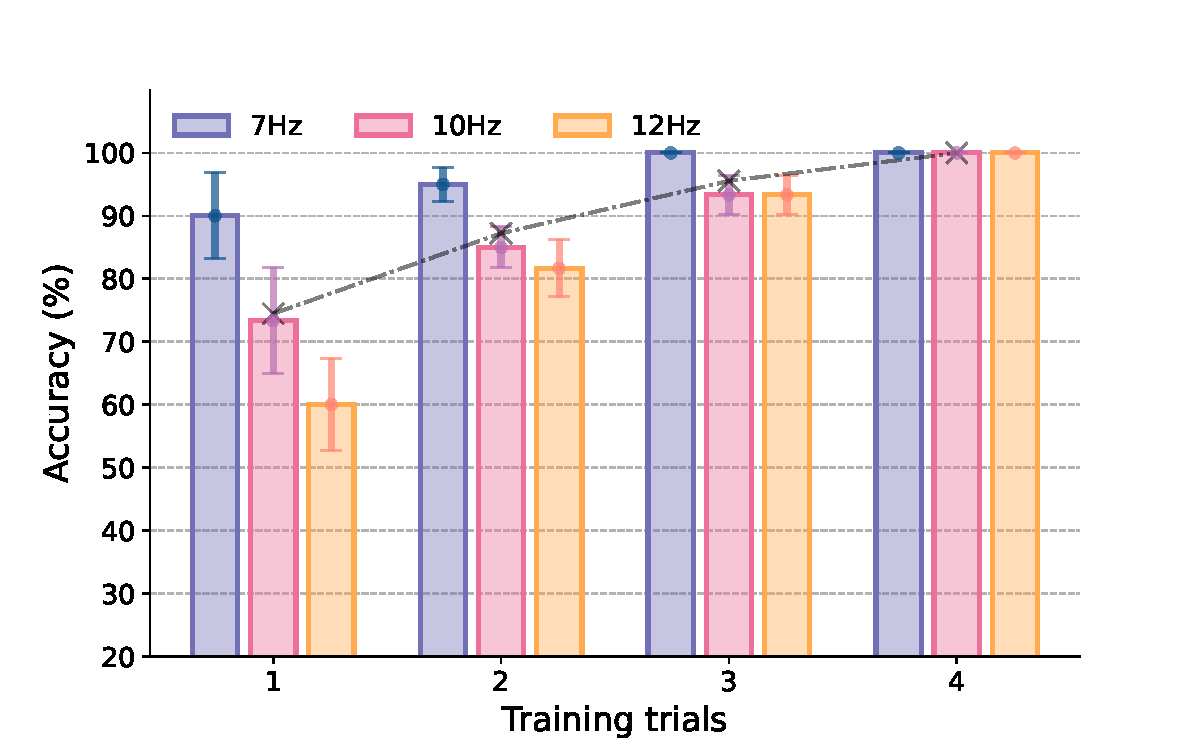
\includegraphics[clip,width=0.49\columnwidth]{report/C6 Results/assets/acc_Nt_mcca_Ns128.pdf}%
%     \label{subfig:mset-nt-ns128}
% }
% \hfill
% \subfloat[$T = 4$s ($N_s=1024, N_s'=256$)]{%
%     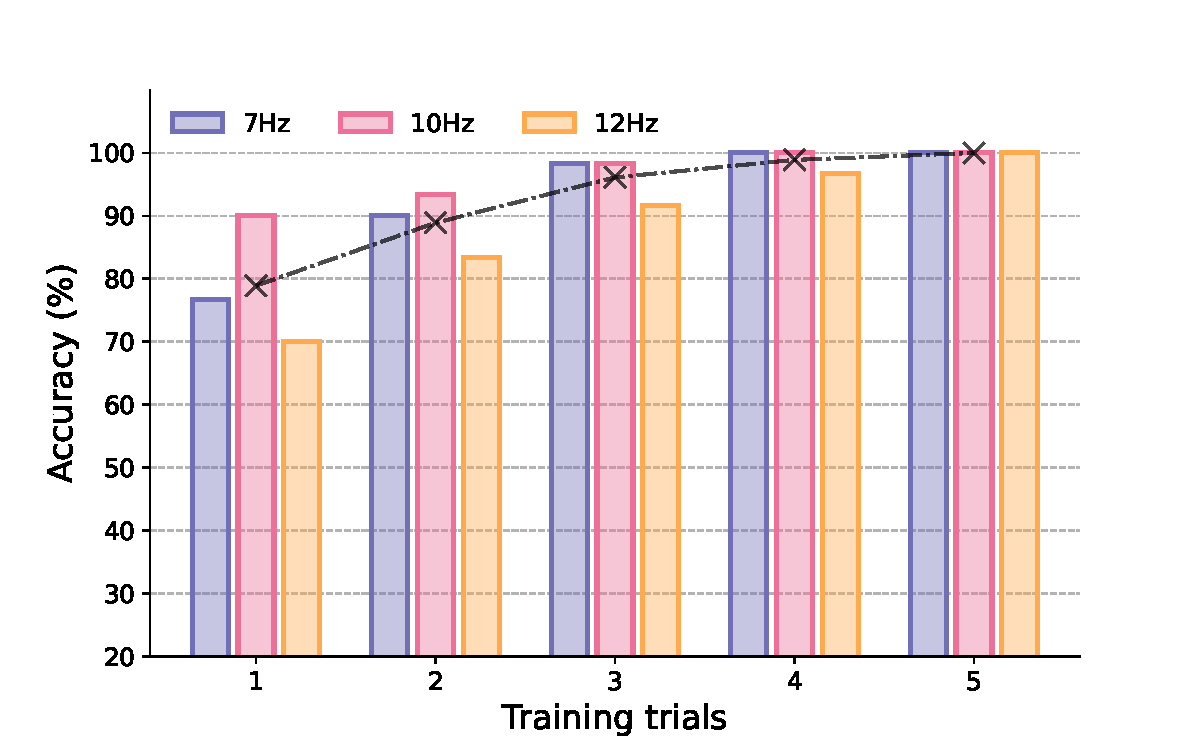
\includegraphics[clip,width=0.49\columnwidth]{report/C6 Results/assets/acc_Nt_mcca_Ns256.pdf}%
%     \label{subfig:mset-nt-ns256}
% }

\caption[MsetCCA decoding accuracy, varying $p$: effect of varying the number of training (calibration) trials $p$ on validation accuracy for recording windows of varying length $T$.]{\textbf{MsetCCA decoding accuracy, varying }$p$: effect of varying the number of training (calibration) trials $p$ on validation accuracy for recording windows of varying length $T$. In each subfigure, all trials are of equal length $T$ seconds which equates to $N_s$ samples at $f_s=256$Hz and $N_s'$ samples at the downsampled rate of $f_s'=64$Hz. Crosses connected with dashed traces denote average decoding accuracy across stimulus frequencies for a given $p=n, \, n\in\{1, \dots, 5\}$. Error bars denote one standard error of the mean.}
\label{fig:mset-acc-nt}
\end{figure}


\begin{figure}[h]

\subfloat[GCCA algorithm]{%
  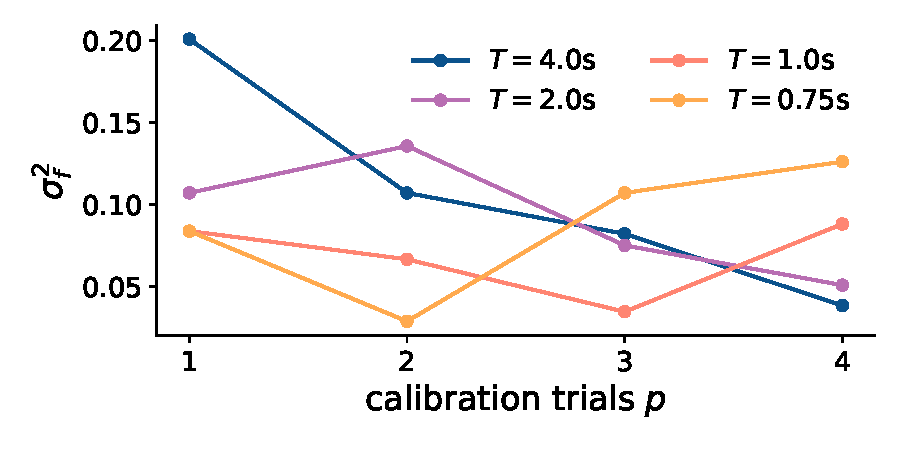
\includegraphics[clip,width=0.46\columnwidth]{report/C6 Results/assets/freq-var-gcca.pdf}%
  \label{subfig:freq-var-gcca}
}
\hfill
\subfloat[MsetCCA algorithm]{%
  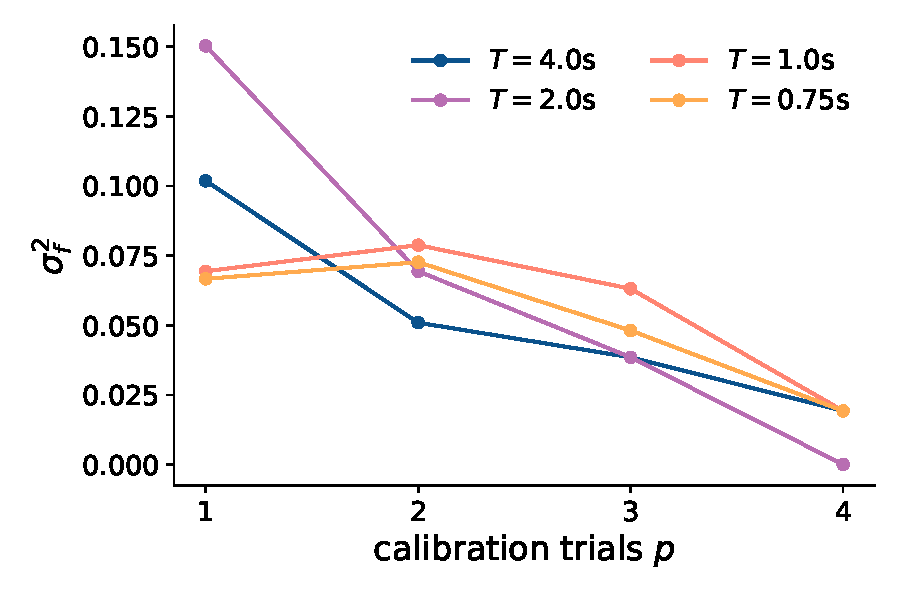
\includegraphics[clip,width=0.46\columnwidth]{report/C6 Results/assets/freq-var-mcca.pdf}%
  \label{subfig:freq-var-mcca}
}
\caption[Graphs showing variance in decoding accuracy across the triad of stimulus frequencies at each value of $p$.]{Graphs showing variance in decoding accuracy across the triad of stimulus frequencies at each value of $p$. The standard deviation in accuracy over frequencies $\sigma_f^2$ is reported. Different colour traces represent recording windows of different lengths as labelled.}
\label{fig:freq-var-plots}
\end{figure}


\subsection{Generalisation testing}
\label{subsection:generalisation-testing}
Of interest to template-based decoding algorithms that leverage historical `training' or calibration data is their ability to \textit{generalise} to new sets of data. In order to clarify this idea in context, consider two trial sessions $X_a$ and $X_b$ taken under \textit{different conditions} where the subject would have at least had to remove and reinstall the BCI headband on their head between sets. Thus, $X_a$ and $X_b$ would be recorded with slightly different electrode positions and contact impedances and would therefore exhibit different signal quality. 

This experiment was thus designed to investigate whether calibration using data from one session, $X_a$ say, would allow generalise to another, say $X_b$. That is, would calibrating using $X_a$ and testing (validating) on $X_b$ yield comparable performance to calibrating and testing on data recorded from the same session as before? If so, the implication is that calibration would only need to be performed once-off, or at least, not \textit{every} recording session which would enhance the user experience. An extension of this experiment was to determine if calibrating using $X_a$ \textit{and} a small subset of $X_b$ and then testing on the remainder of $X_b$ would yield better performance than only calibrating on the subset of $X_b$ as in previous experiments.

The results of such an experiment are shown in Figure \ref{fig:gt-results-gcca} and Figure \ref{fig:gt-results-mcca} for the GCCA and MsetCCA algorithms respectively. Continuing the analogy with $X_a$ and $X_b$ above, the number of `overlapping trials' in these figures refers to the number of trials from $X_b$ included in the calibration set along with the whole of $X_a$. Accordingly, 0 overlapping trials would correspond to a situation where calibration was performed exclusively on $X_a$ and testing on $X_b$. This condition tests the initial question in the experiment mentioned above. The case of $n$ overlapping trials with $x>1$ corresponds to calibration using all of $X_a$ \textit{and} $n$ trials from $X_b$ while still testing using the left-over\footnote{the set difference between all trials in $X_b$ and the $n$-element subset used for calibration.} trials from $X_b$. Calibration and `training`, as referred to in the figures, are used interchangeably here.

%% [GENERALISATION] Experiments with varying Ns: GCCA
\begin{figure}[!htb]
\subfloat[$N_s=512, \, N_s'=128 \, \Leftrightarrow T = 2$s ]{%
    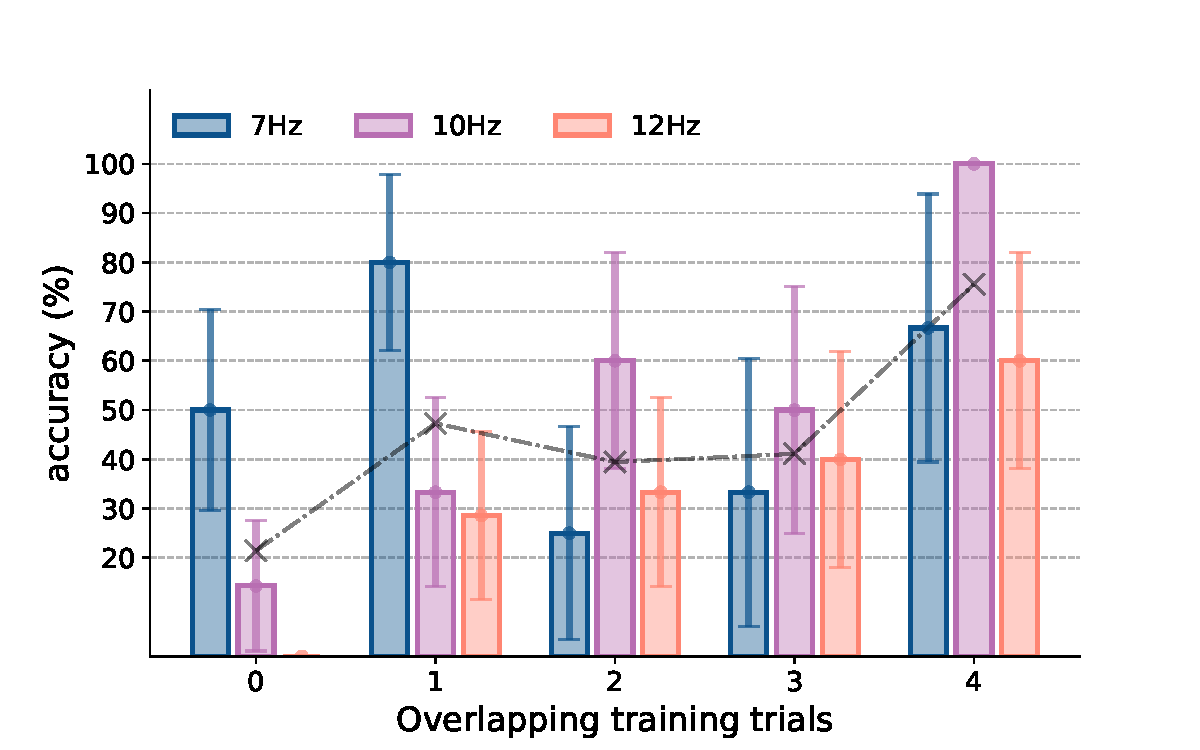
\includegraphics[clip,width=0.49\columnwidth]{report/C6 Results/assets/gt_acc_gcca_Ns128.pdf}%
    \label{subfig:gt-gcca-ns128}
}
\hfill
\subfloat[$N_s=1024, \, N_s'=256 \, \Leftrightarrow T = 4$s]{%
    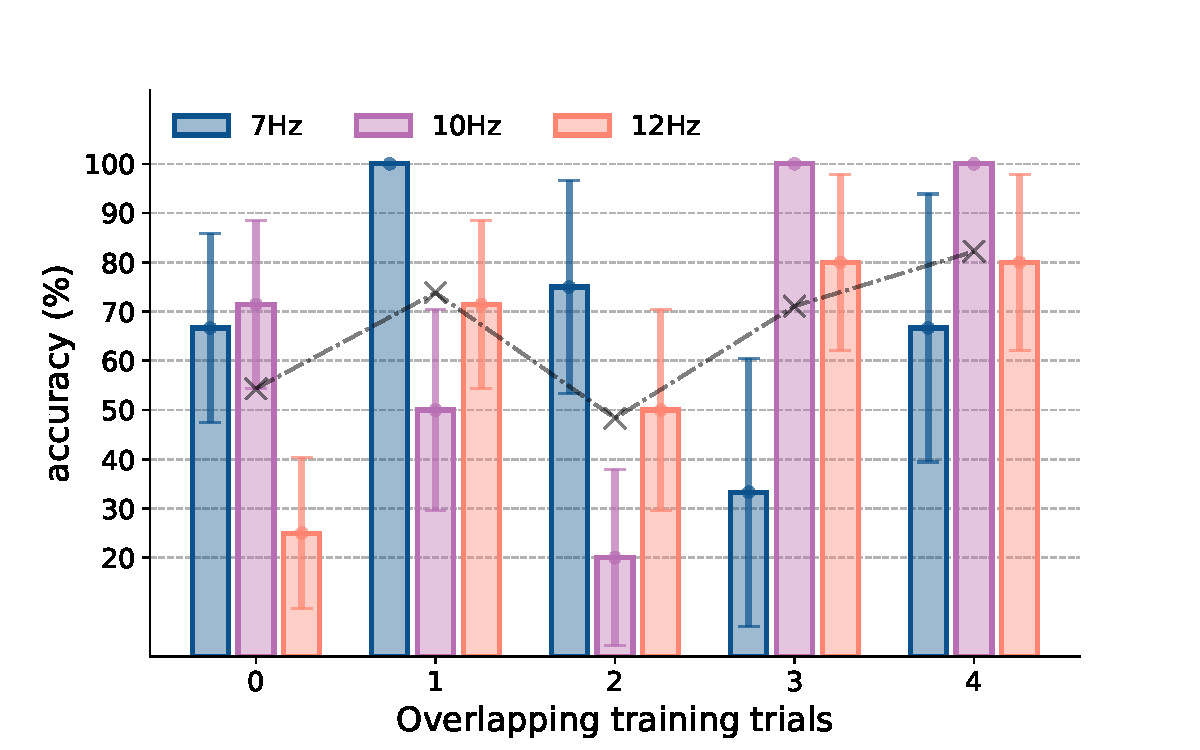
\includegraphics[clip,width=0.49\columnwidth]{report/C6 Results/assets/gt_acc_gcca_Ns256.pdf}%
    \label{subfig:gt-gcca-ns256}
}
\caption[GCCA generalisation performance: test decoding accuracy when calibrating and testing on data collected from distinct sessions under different conditions]{\textbf{GCCA generalisation performance}: decoding accuracy on data from distinct recording sessions taken under different conditions, $X_a$ and $X_b$ where $X_a$ is a calibration (training) set and $X_b$ a test set. The number of overlapping trials refers to the number of trials in $X_b$ \textit{also} used for calibration. Results using $T=2$s and $T=4$s recording windows are shown. Error bars denote one standard error of the mean.}
\label{fig:gt-results-gcca}
\end{figure}

%% [GENERALISATION] Experiments with varying Ns: MsetCCA
\begin{figure}[!htb]
\subfloat[$N_s=512, \, N_s'=128 \, \Leftrightarrow T = 2$s]{%
    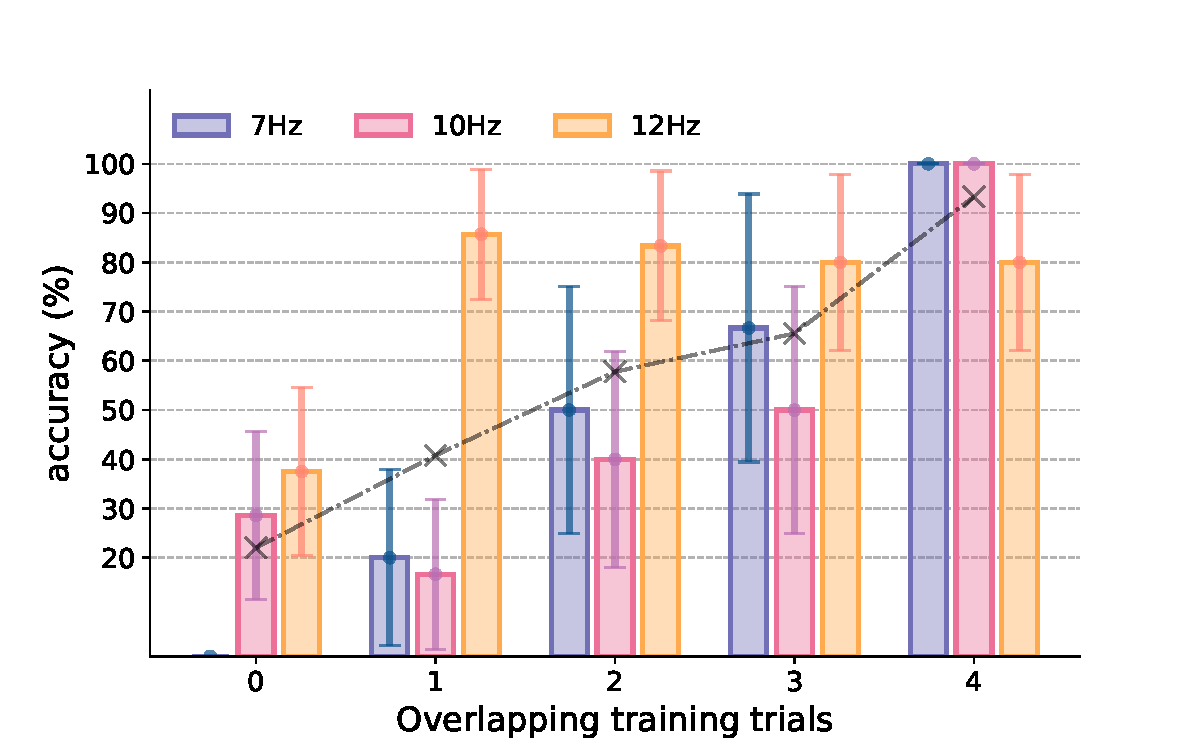
\includegraphics[clip,width=0.49\columnwidth]{report/C6 Results/assets/gt_acc_mcca_Ns128.pdf}%
    \label{subfig:gt-mcca-ns128}
}
\hfill
\subfloat[$N_s=1024, \, N_s'=256 \, \Leftrightarrow T = 4$s ]{%
    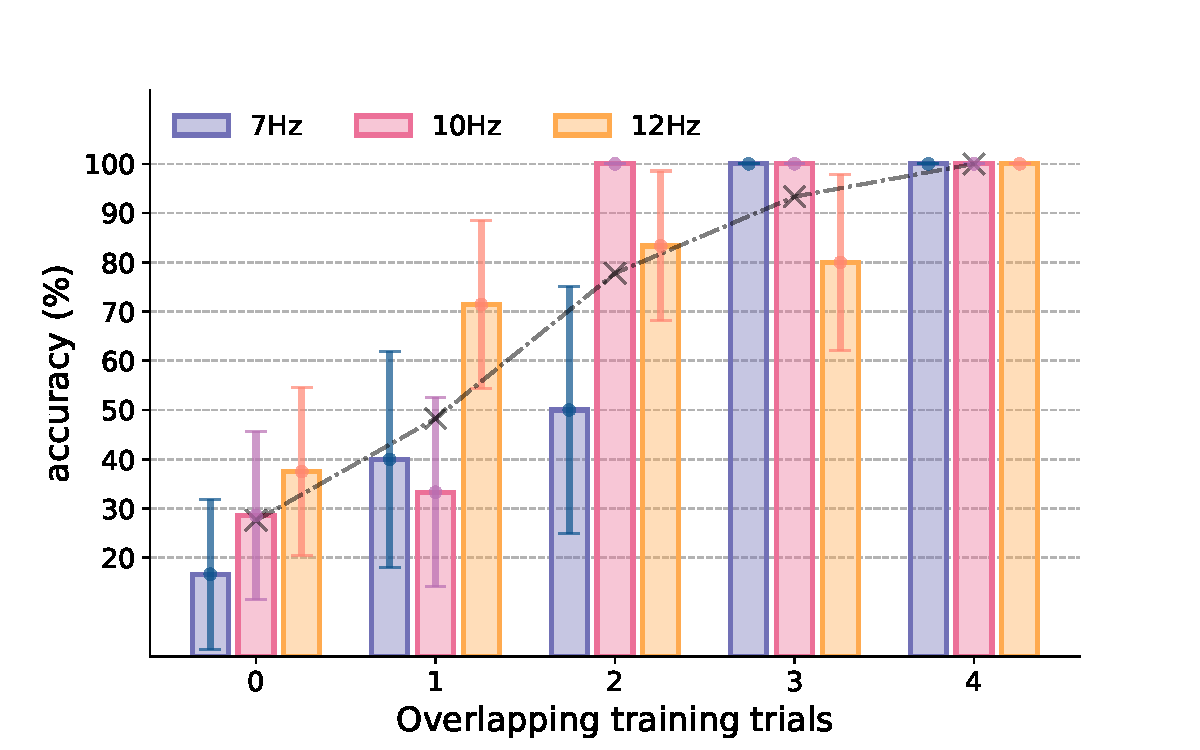
\includegraphics[clip,width=0.49\columnwidth]{report/C6 Results/assets/gt_acc_mcca_Ns256.pdf}%
    \label{subfig:gt-mcca-ns256}
}
\caption[MsetCCA generalisation performance: test decoding accuracy when calibrating and testing on data collected from distinct sessions under different conditions]{\textbf{MsetCCA generalisation performance}: decoding accuracy on data from distinct recording sessions taken under different conditions, $X_a$ and $X_b$ where $X_a$ is a calibration (training) set and $X_b$ a test set. The number of overlapping trials refers to the number of trials in $X_b$ \textit{also} used for calibration. Results using $T=2$s and $T=4$s recording windows are shown. Error bars denote one standard error of the mean.}
\label{fig:gt-results-mcca}
\end{figure}


\begin{table}[]
\centering
\resizebox{\textwidth}{!}{%
\begin{tabular}{@{}lllllllllllllllll@{}}
\toprule
\textbf{$p$} &
  \multicolumn{4}{c}{\textbf{1}} &
  \multicolumn{4}{c}{\textbf{2}} &
  \multicolumn{4}{c}{\textbf{3}} &
  \multicolumn{4}{c}{\textbf{4}} \\ \midrule
\textbf{$T$} &
  \multicolumn{1}{c}{\textbf{0.75}} &
  \multicolumn{1}{c}{\textbf{1}} &
  \multicolumn{1}{c}{\textbf{2}} &
  \multicolumn{1}{c}{\textbf{4}} &
  \multicolumn{1}{c}{\textbf{0.75}} &
  \multicolumn{1}{c}{\textbf{1}} &
  \multicolumn{1}{c}{\textbf{2}} &
  \multicolumn{1}{c}{\textbf{4}} &
  \multicolumn{1}{c}{\textbf{0.75}} &
  \multicolumn{1}{c}{\textbf{1}} &
  \multicolumn{1}{c}{\textbf{2}} &
  \multicolumn{1}{c}{\textbf{4}} &
  \multicolumn{1}{c}{\textbf{0.75}} &
  \multicolumn{1}{c}{\textbf{1}} &
  \multicolumn{1}{c}{\textbf{2}} &
  \multicolumn{1}{c}{\textbf{4}} \\ \cmidrule(l){2-17} 
$\mathbf{\bar{x}}$ &
  52.22 &
  65.56 &
  72.22 &
  74.44 &
  63.33 &
  71.67 &
  83.89 &
  90.56 &
  71.11 &
  82.78 &
  91.11 &
  94.44 &
  77.78 &
  83.33 &
  95.56 &
  \textbf{97.78} \\
$\mathbf{s_{\bar{x}}}$ &
  8.341 &
  7.800 &
  6.204 &
  7.120 &
  6.037 &
  5.292 &
  3.590 &
  2.823 &
  5.095 &
  4.556 &
  3.167 &
  1.824 &
  7.098 &
  6.558 &
  2.893 &
  \textbf{1.514} \\
$\boldsymbol{\sigma_f}^2$ &
  0.084 &
  0.084 &
  0.107 &
  0.201 &
  \textbf{0.029} &
  0.067 &
  0.136 &
  0.107 &
  0.107 &
  0.035 &
  0.075 &
  0.082 &
  0.126 &
  0.088 &
  0.051 &
  0.039 \\
 \textbf{ITR} &
  8.69 &
  18.70 &
  13.64 &
  7.64 &
  21.61 &
  26.51 &
  23.61 &
  15.59 &
  34.30 &
  45.00 &
  31.90 &
  18.29 &
  \textbf{47.89} &
  46.09 &
  38.35 &
  21.14 \\ \bottomrule
\end{tabular}%
}
\caption[GCCA results summary: a compilation of decoding performance metrics for the GCCA algorithm.]{\textbf{GCCA results summary}: a compilation of decoding performance metrics for the GCCA algorithm. Results are reported over varying numbers of calibration trials $p$ and recording window lengths $T$ (in seconds). Average accuracy across frequency $\mathbf{\bar{x}}$ its standard error $\mathbf{s_{\bar{x}}}$ are reported in $\%$. \textbf{ITR} is given in bits/min. Frequency variance $\boldsymbol{\sigma_f}^2$ is dimensionless.}
\label{tab:gcca-results}
\end{table}

\begin{table}[]
\centering
\small
\resizebox{\textwidth}{!}{%
\begin{tabular}{@{}lllllllllllllllll@{}}
\toprule
$p$          & \multicolumn{4}{c}{\textbf{1}} & \multicolumn{4}{c}{\textbf{2}} & \multicolumn{4}{c}{\textbf{3}} & \multicolumn{4}{c}{\textbf{4}} \\ \midrule
$T$ &
  \textbf{0.75} &
  \textbf{1} &
  \textbf{2} &
  \textbf{4} &
  \textbf{0.75} &
  \textbf{1} &
  \textbf{2} &
  \textbf{3} &
  \textbf{0.75} &
  \textbf{1} &
  \textbf{2} &
  \textbf{4} &
  \textbf{0.75} &
  \textbf{1} &
  \textbf{2} &
  \textbf{4} \\ \cmidrule(l){2-17} 
$\mathbf{\bar{x}}$ & 60.00  & 64.44 & 74.44 & 78.89 & 76.67  & 80.56 & 87.22 & 88.89 & 88.89  & 90.56 & 95.56 & 96.11 & 95.56  & 95.56 & 98.89 & \textbf{98.89} \\
$\mathbf{s_{\bar{x}}}$  & 7.070  & 8.341 & 7.522 & 7.659 & 4.633  & 4.462 & 3.496 & 3.126 & 3.716  & 3.438 & 2.039 & 2.215 & 3.736  & 3.736 & \textbf{0.512} & 1.111 \\
$\boldsymbol{\sigma_f}^2$ & 0.067  & 0.069 & 0.150 & 0.102 & 0.073  & 0.079 & 0.069 & 0.051 & 0.048  & 0.063 & 0.039 & 0.039 & 0.019  & 0.019 & 0.019 & \textbf{0.019} \\
\textbf{ITR} & 17.12  & 17.42 & 15.28 & 9.45  & 45.44  & 40.80 & 27.17 & 14.56 & 77.65  & 62.37 & 38.35 & 19.63 & \textbf{102.28} & 76.71 & 44.58 & 22.29 \\ \bottomrule
\end{tabular}%
}
\caption[MsetCCA results summary: a compilation of decoding performance metrics for the MsetCCA algorithm.]{\textbf{MsetCCA results summary}: a compilation of decoding performance metrics for the MsetCCA algorithm. Results are reported over varying numbers of calibration trials $p$ and recording window lengths $T$ (in seconds). Average accuracy across frequency $\mathbf{\bar{x}}$ its standard error $\mathbf{s_{\bar{x}}}$ are reported in $\%$. \textbf{ITR} is given in bits/min. Frequency variance $\boldsymbol{\sigma_f}^2$ is dimensionless.}
\label{tab:mcca-results}
\end{table}


% \begin{figure}
%      \centering
%      \begin{subfigure}[b]{0.3\textwidth}
%          \centering
%          \includegraphics[width=\textwidth]{acc}
%          \caption{$y=x$}
%          \label{fig:y equals x}
%      \end{subfigure}
%      \hfill
%      \begin{subfigure}[b]{0.3\textwidth}
%          \centering
%          \includegraphics[width=\textwidth]{graph2}
%          \caption{$y=3sinx$}
%          \label{fig:three sin x}
%      \end{subfigure}
%      \hfill
%      \begin{subfigure}[b]{0.3\textwidth}
%          \centering
%          \includegraphics[width=\textwidth]{graph3}
%          \caption{$y=5/x$}
%          \label{fig:five over x}
%      \end{subfigure}
%         \caption{Three simple graphs}
%         \label{fig:three graphs}
% \end{figure}

% \section{Experiments using Benchmark Data}
